

\section{Shape Analysis and Statistical Approach \label{sec:shape}}

In order to test the utility of the super-razor kinematic variables in the context of a search for slepton and chargino production we consider toy experimental analyses. Each of these analyses is a shape analysis, using multiple bins over the range of a kinematic variable of interest, and exploiting differences in changing signal and background expectations over the bins. This approach is used to increase the information being gleaned from these kinematic variables, allowing us to quantify what the maximal performance could look like, irrespective of changing optimized cuts associated with coarser binning. The predictions of these toy shape analyses are potentially optimistic relative to CMS and ATLAS results, due to both increased complexity of the analyses and the shortcomings of the detector simulation utilized here. To account for these differences, large systematic uncertainties are included in the procedure to represent potential experimental uncertainty in the relevant parameters that dictate the shape and yield of signal and background events.

\subsection{Analysis strategy}

For each toy analysis there are one or more kinematic variables identified as the discriminating variable, and the binned distribution of event yields in this variable are the observables in the toy experiment. The expected shape of both signal and background in the variable(s) of interest are required input for this procedure for each process. In our case, these shapes come from simulated event samples of each process. For an actual experimental analysis some can be measured or constrained from control regions. Regardless of their provenance, the uncertainties corresponding to these shapes are as important as the central values as we try to reflect in these toy analyses.

For the CMS and ATLAS analyses, control regions are identified using both object ID and kinematic information in order to isolate particular backgrounds. $Z$ mass windows are used to select $(Z/\gamma^*\to \ell\ell)$+jets backgrounds for normalizing $Z$ mass veto signal regions. Similarly, high jet multiplicity or $b$-tagged jet-enriched selections are used to constrain backgrounds with top quarks. In order to qualitatively capture these control region background constraints we consider multiple lepton flavor ($ee$, $e\mu$, $\mu\mu$) and jet multiplicity ($0$, $1$, $\ge 2$) categories simultaneously in a fit to data, with binned kinematic discriminants for each category. In each fit, high jet multiplicity categories effectively constrain top contributions while di-boson and $Z/\gamma^*$ events at low jet multiplicity are disentangled using relative lepton flavor category yields.

We first consider one-dimensional analyses, where the kinematic discriminant is chosen to be $M_{\Delta}^{R}$, $M_{CT\perp}$ or $M_{T2}$. The distribution of the variable of interest is binned in 10 GeV steps from zero to 500 GeV. Only events satisfying the baseline selection and the relevant CMS (for $M_{CT\perp}$) or ATLAS (for $M_{T2}$) selection are included. The expected $M_{\Delta}^{R}$ and $M_{T2}$ distributions in the $ee$ final state for sample di-slepton signals and backgrounds are shown in Figure~\ref{fig:EEPDF}. We observe the changing background compositions and diminishing expected signal yield with increasing jet multiplicity. Distributions for each of the $M_{\Delta}$-sensitive variables and selections considered are shown for the $e\mu$, $N_{jet}=0$ final state in Figure~\ref{fig:EMUPDF}.

\begin{figure}[ht]
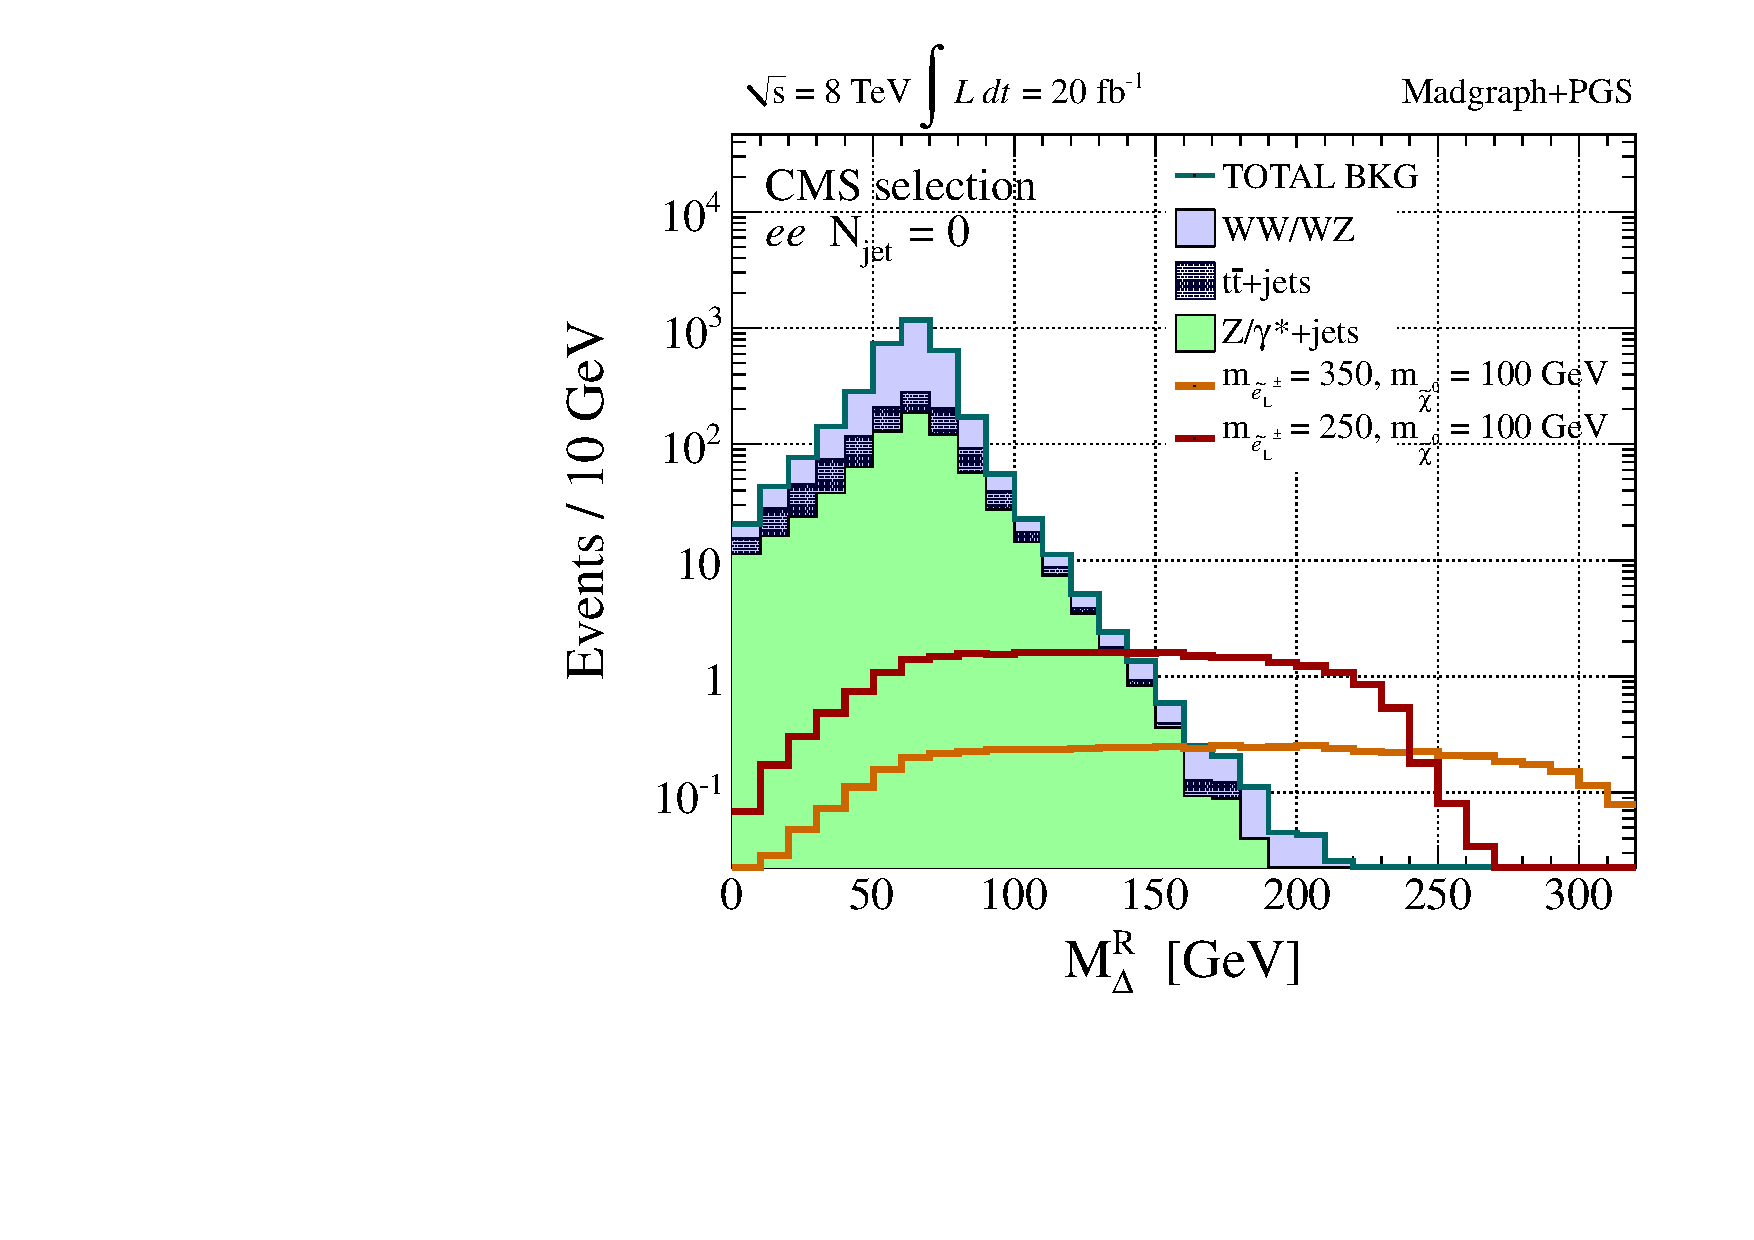
\includegraphics[width=0.3\columnwidth]{fig/sectionIV/PDF_selectronL_CMS_Mdelta_ee_Njet0.pdf}
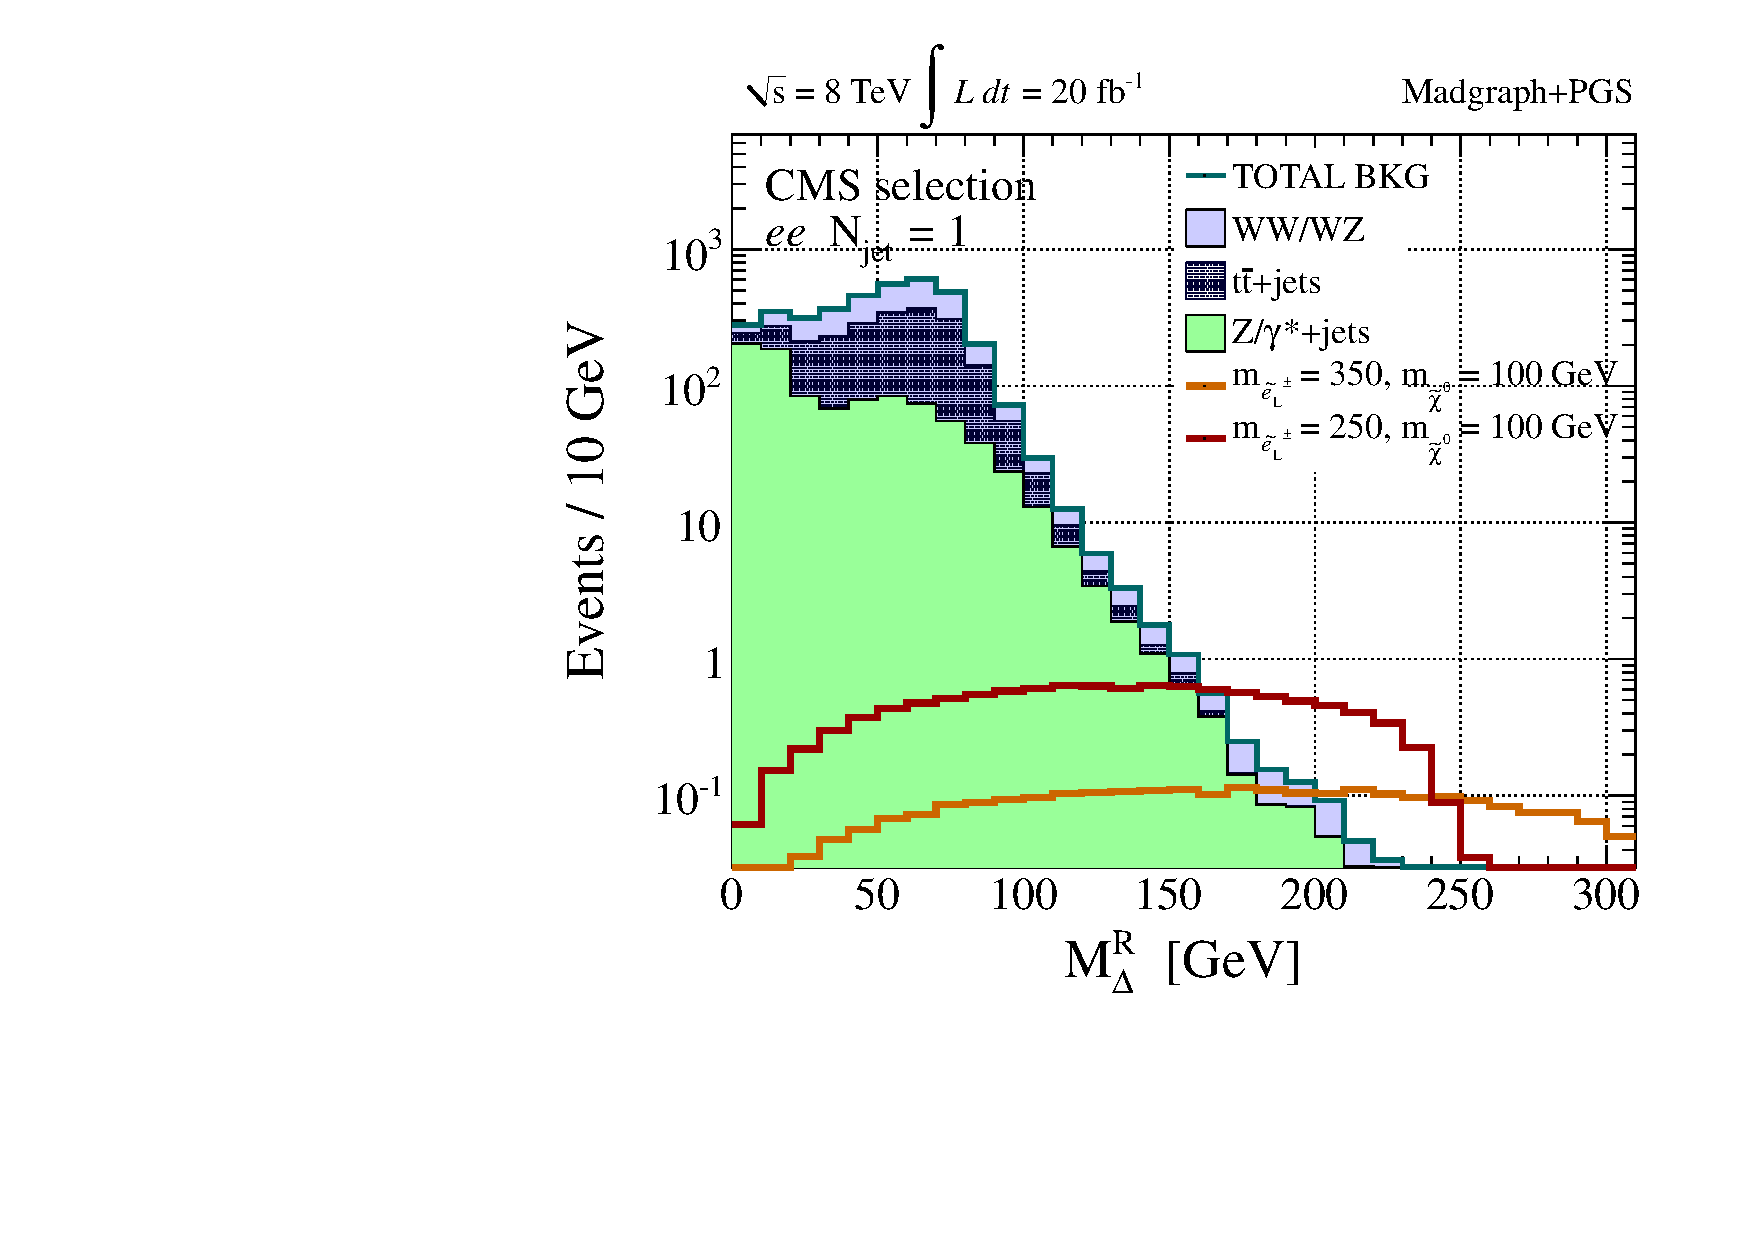
\includegraphics[width=0.3\columnwidth]{fig/sectionIV/PDF_selectronL_CMS_Mdelta_ee_Njet1.pdf}
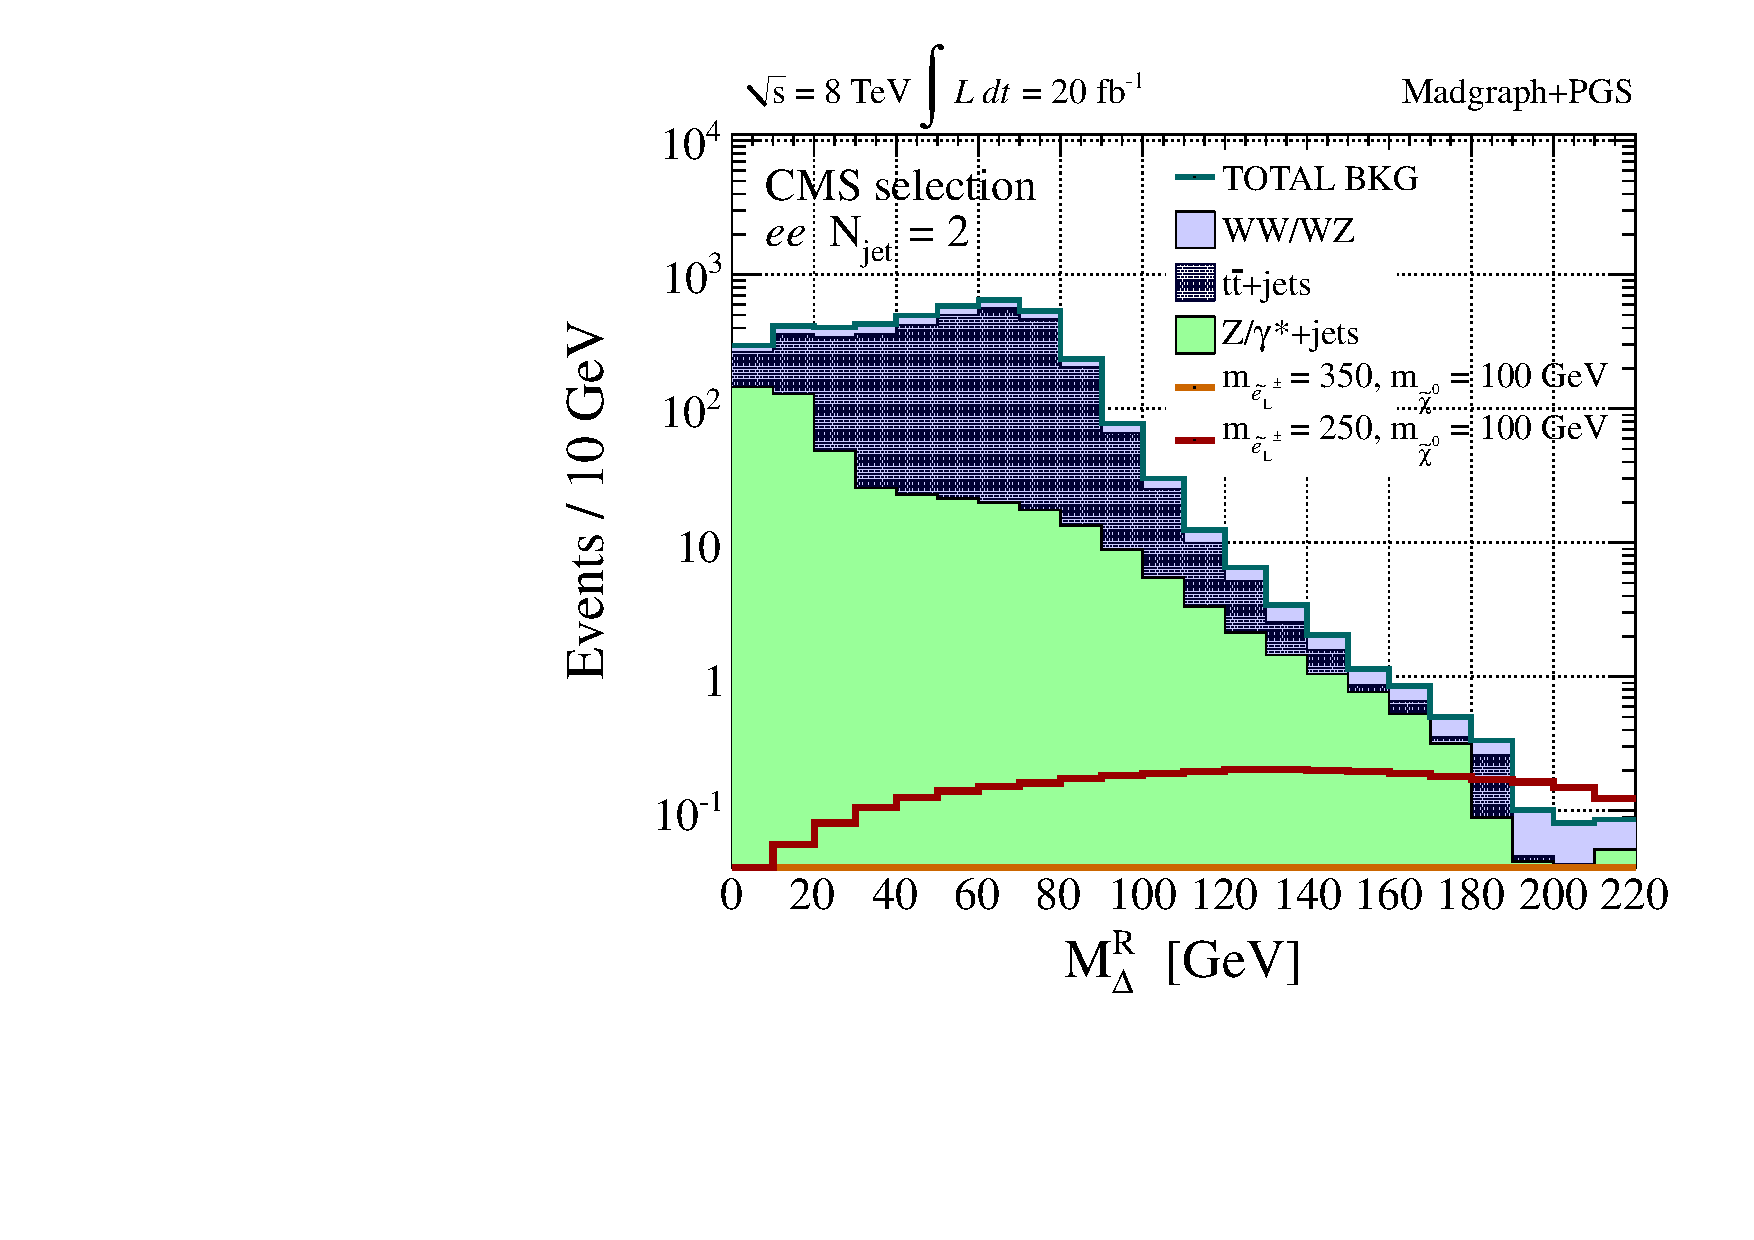
\includegraphics[width=0.3\columnwidth]{fig/sectionIV/PDF_selectronL_CMS_Mdelta_ee_Njet2.pdf}
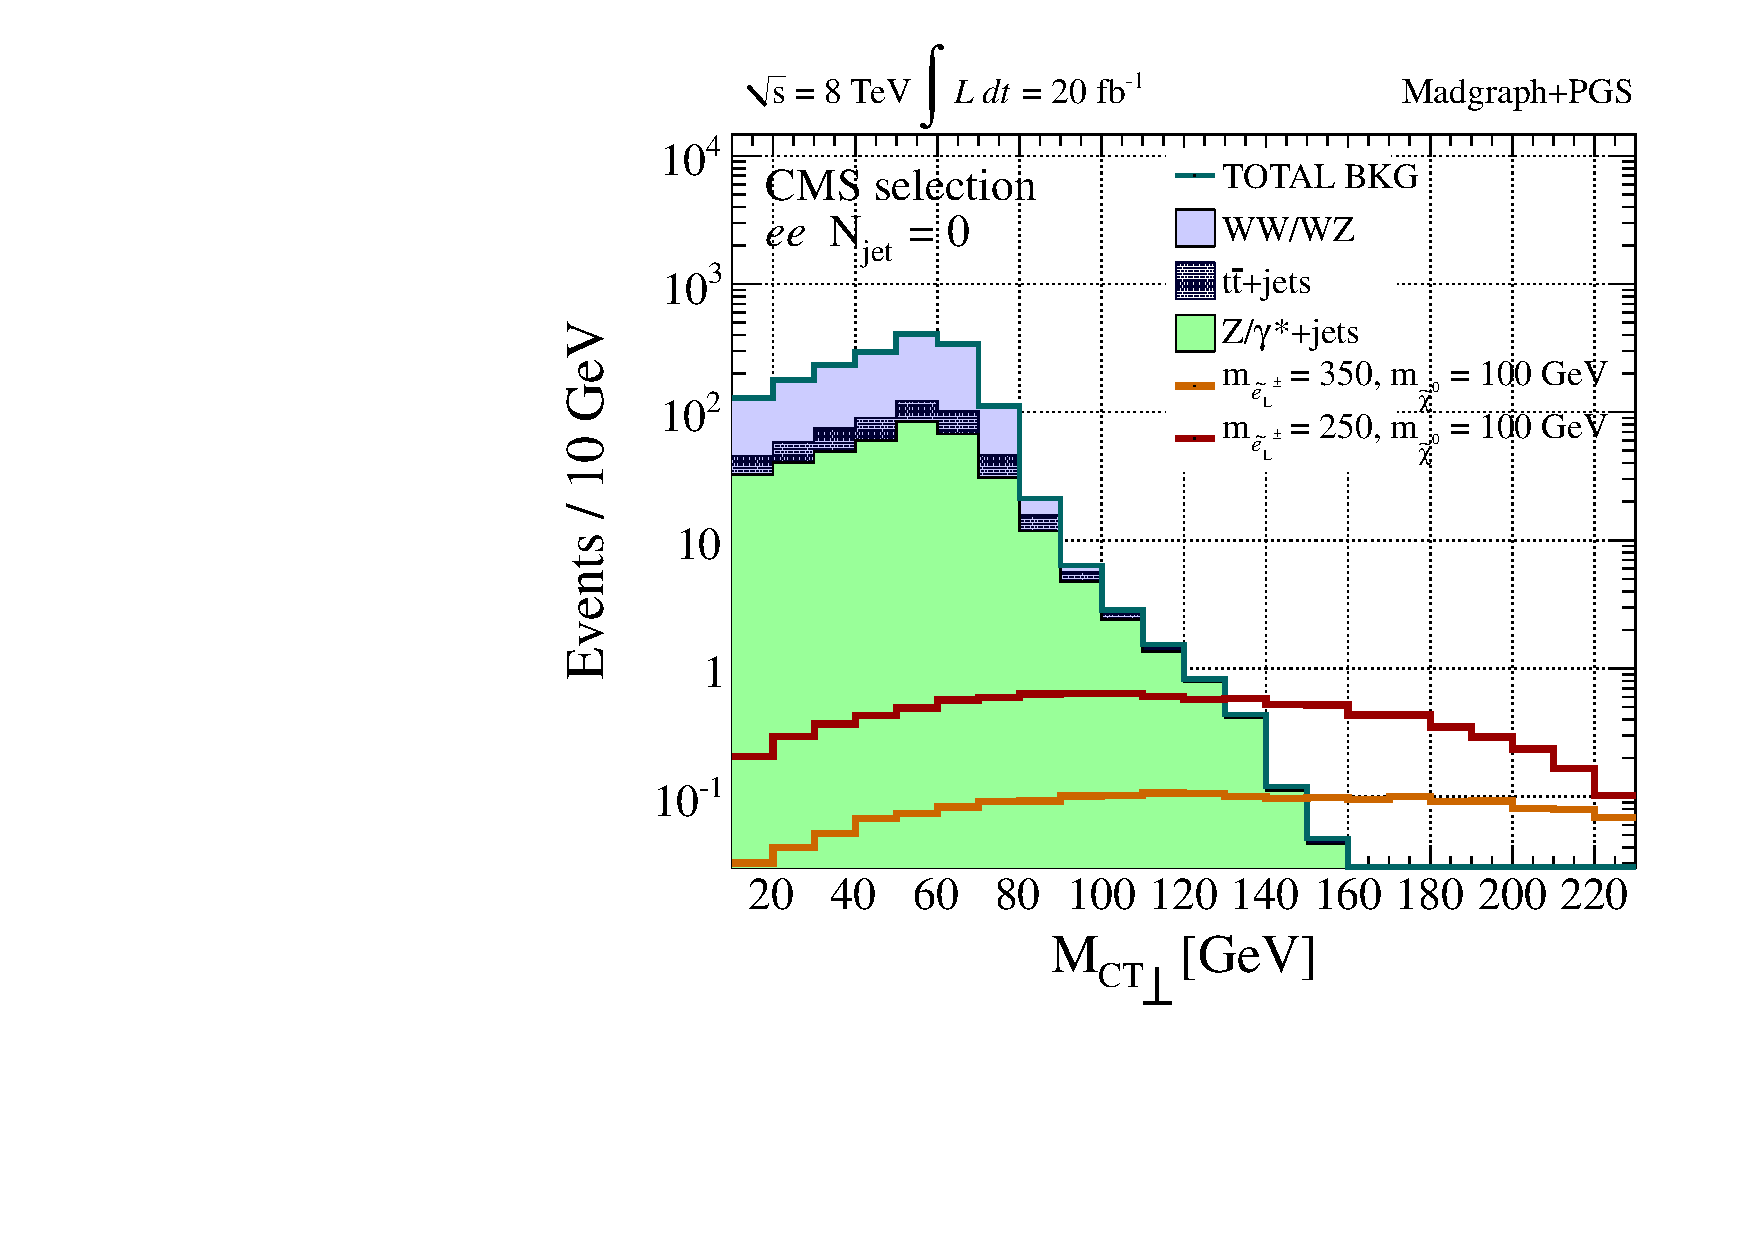
\includegraphics[width=0.3\columnwidth]{fig/sectionIV/PDF_selectronL_CMS_MCTperp_ee_Njet0.pdf}
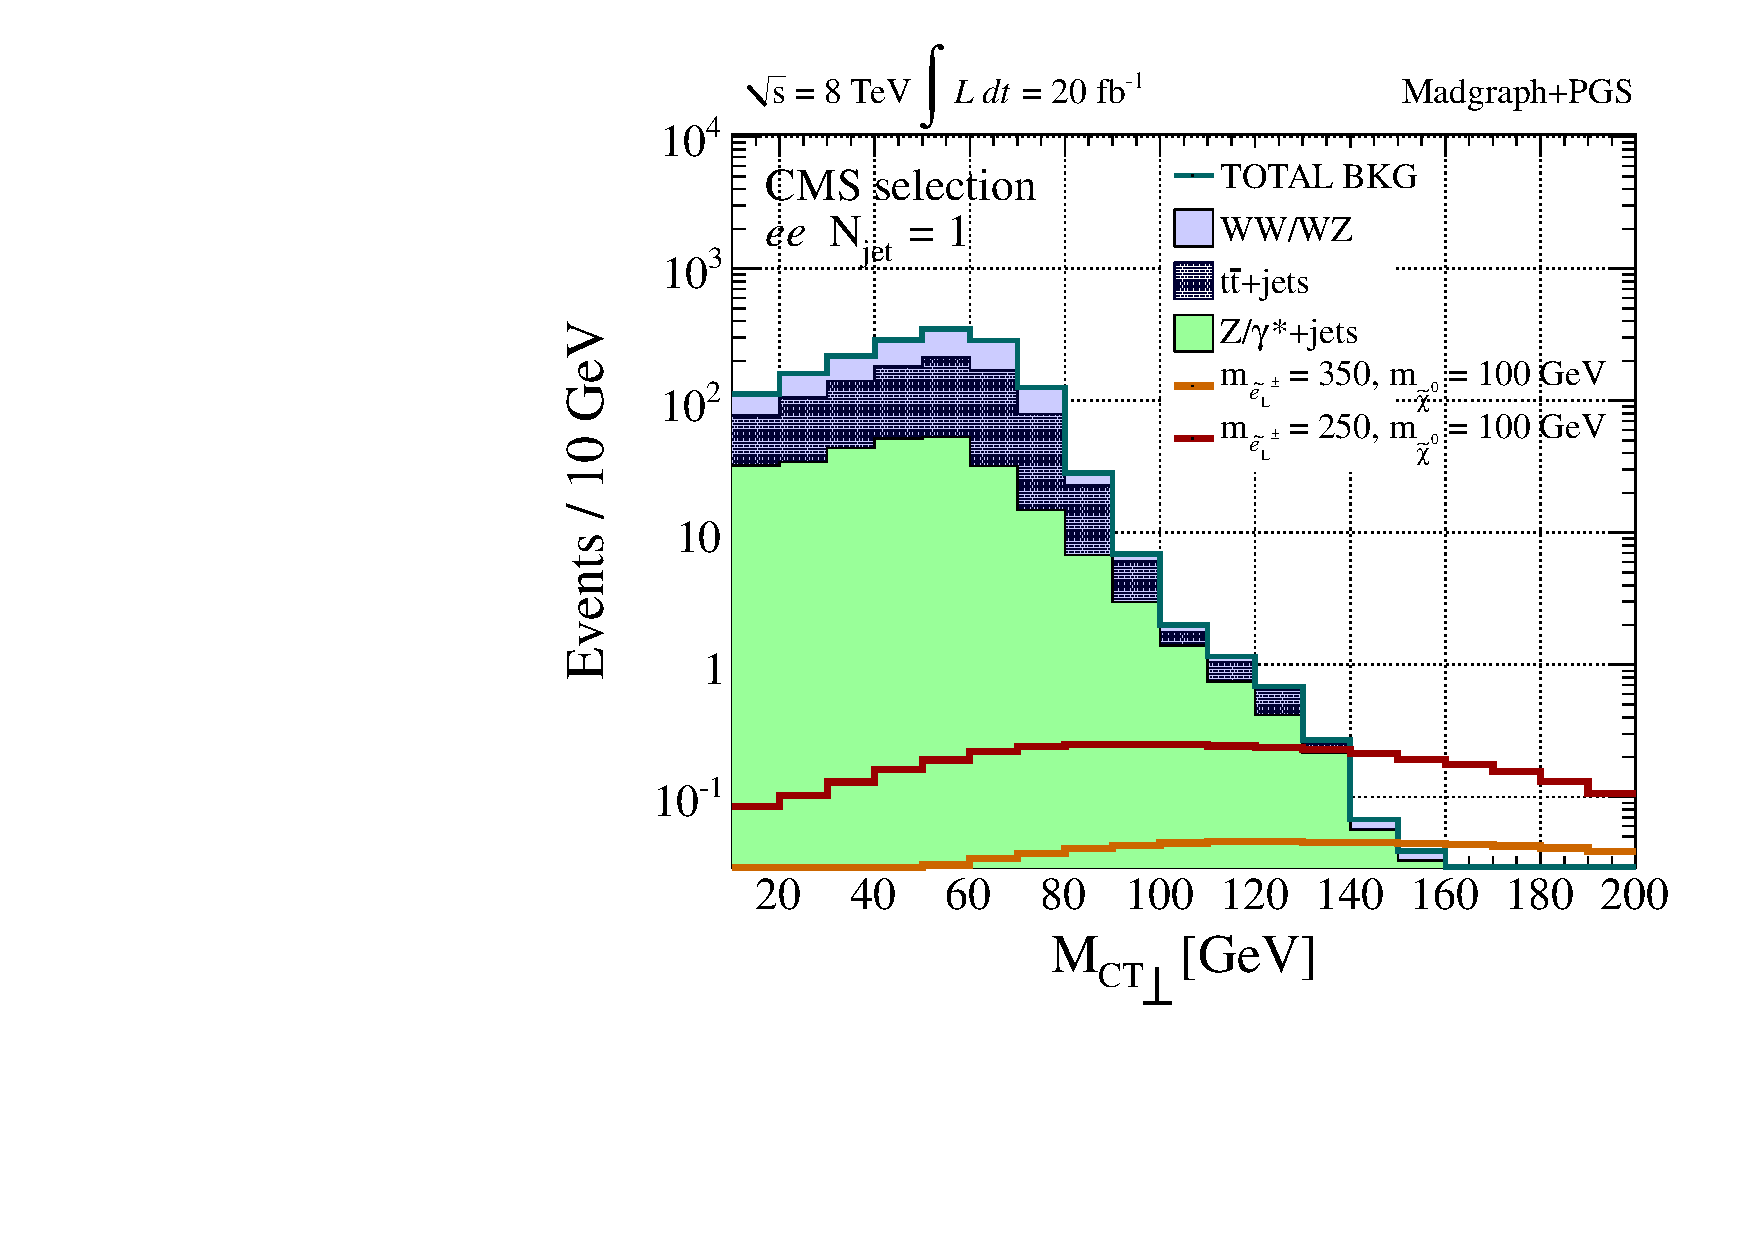
\includegraphics[width=0.3\columnwidth]{fig/sectionIV/PDF_selectronL_CMS_MCTperp_ee_Njet1.pdf}
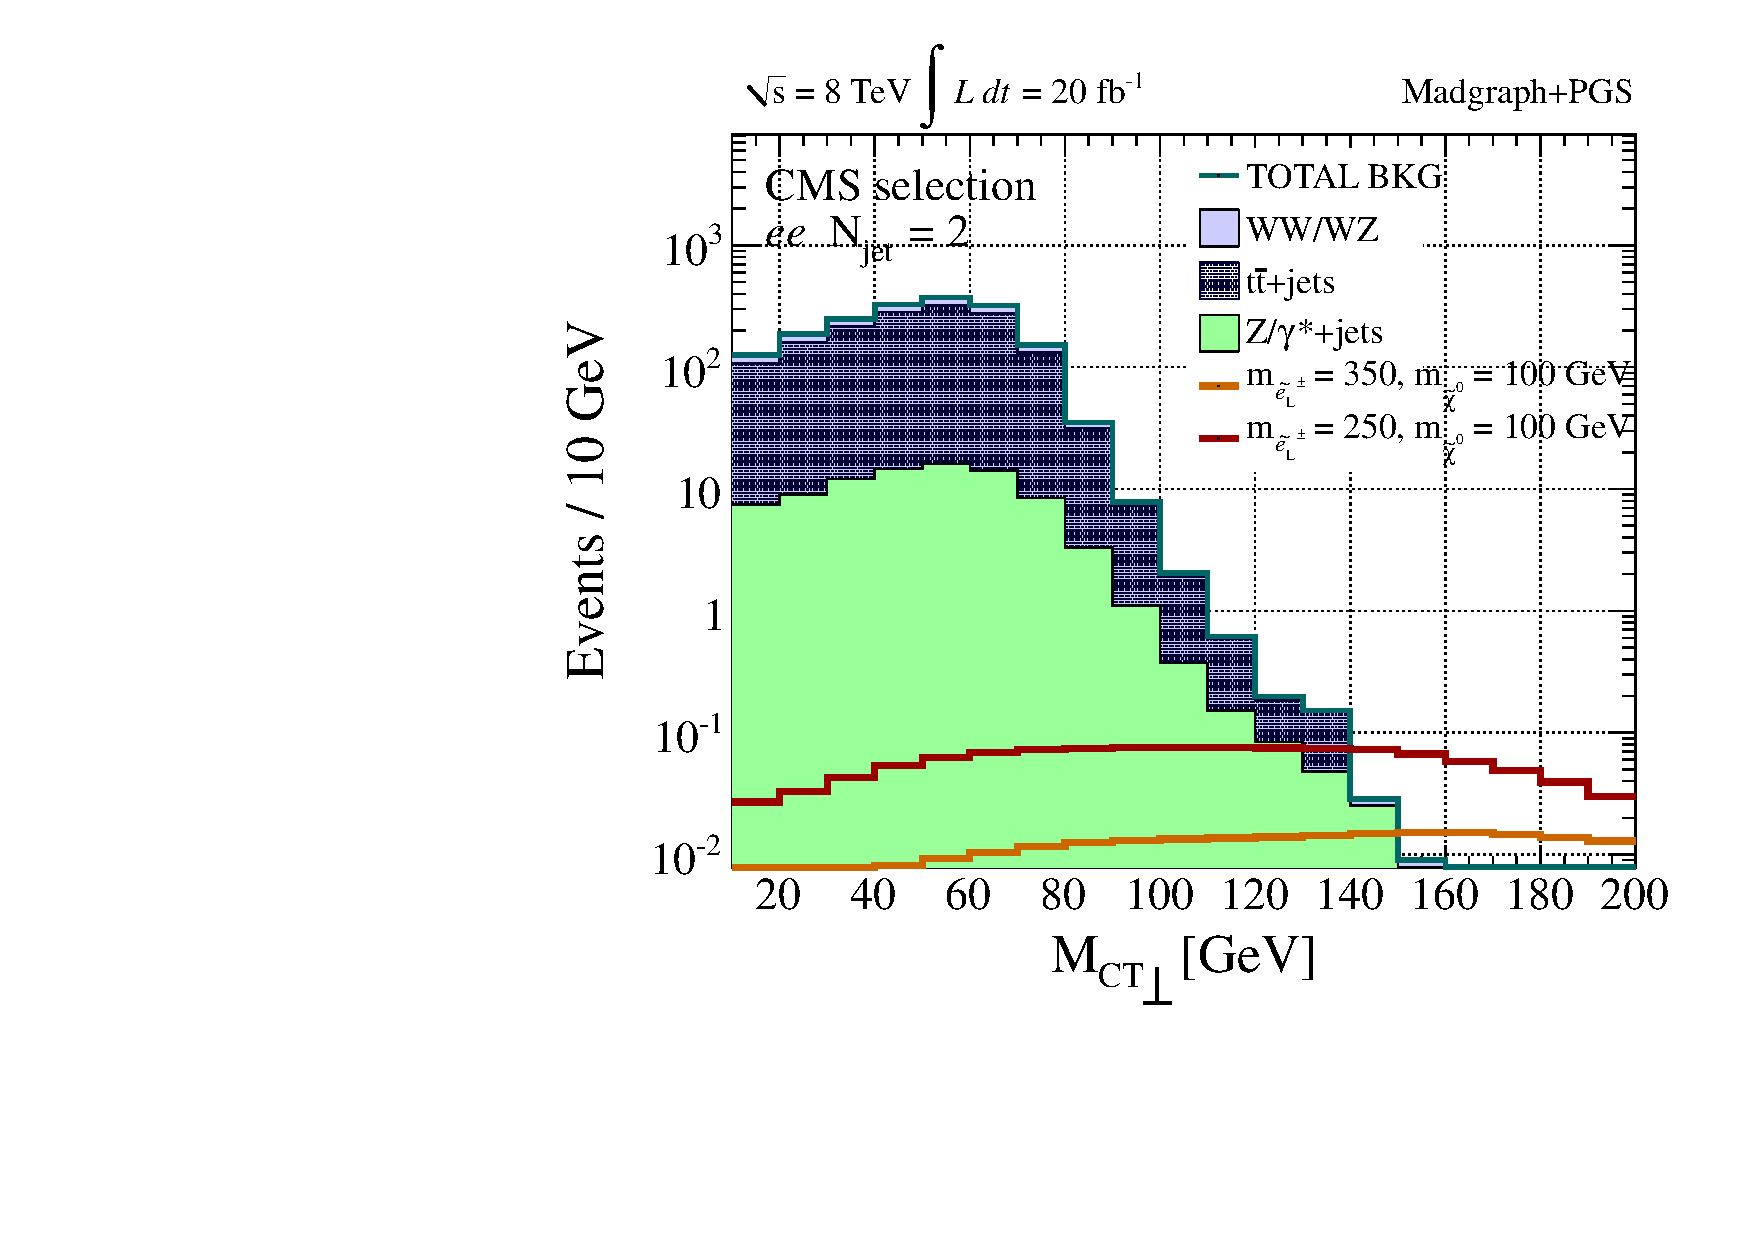
\includegraphics[width=0.3\columnwidth]{fig/sectionIV/PDF_selectronL_CMS_MCTperp_ee_Njet2.pdf}
\caption{Expected background yields in the $ee$ final state passing the CMS selection, normalized to 20 fb$^{-1}$ of data, for different jet multiplicities. Sample left-handed di-selectron signals are included with ($m_{\tilde{\ell}_{L}} = 350$,~$m_{\tilde{\chi}_{1}^0} = 100$) and ($m_{\tilde{\ell}_{L}} = 250$,~$m_{\tilde{\chi}_{1}^0} = 100$)~GeV. Top: $M_{\Delta}^{R}$ distribution. Bottom: $M_{CT\perp}$ distribution. Left: $N_{jet} = 0$. Center: $N_{jet} = 1$. Right: $N_{jet} \ge 2$. \label{fig:EEPDF}}
\end{figure}

\begin{figure}[ht]
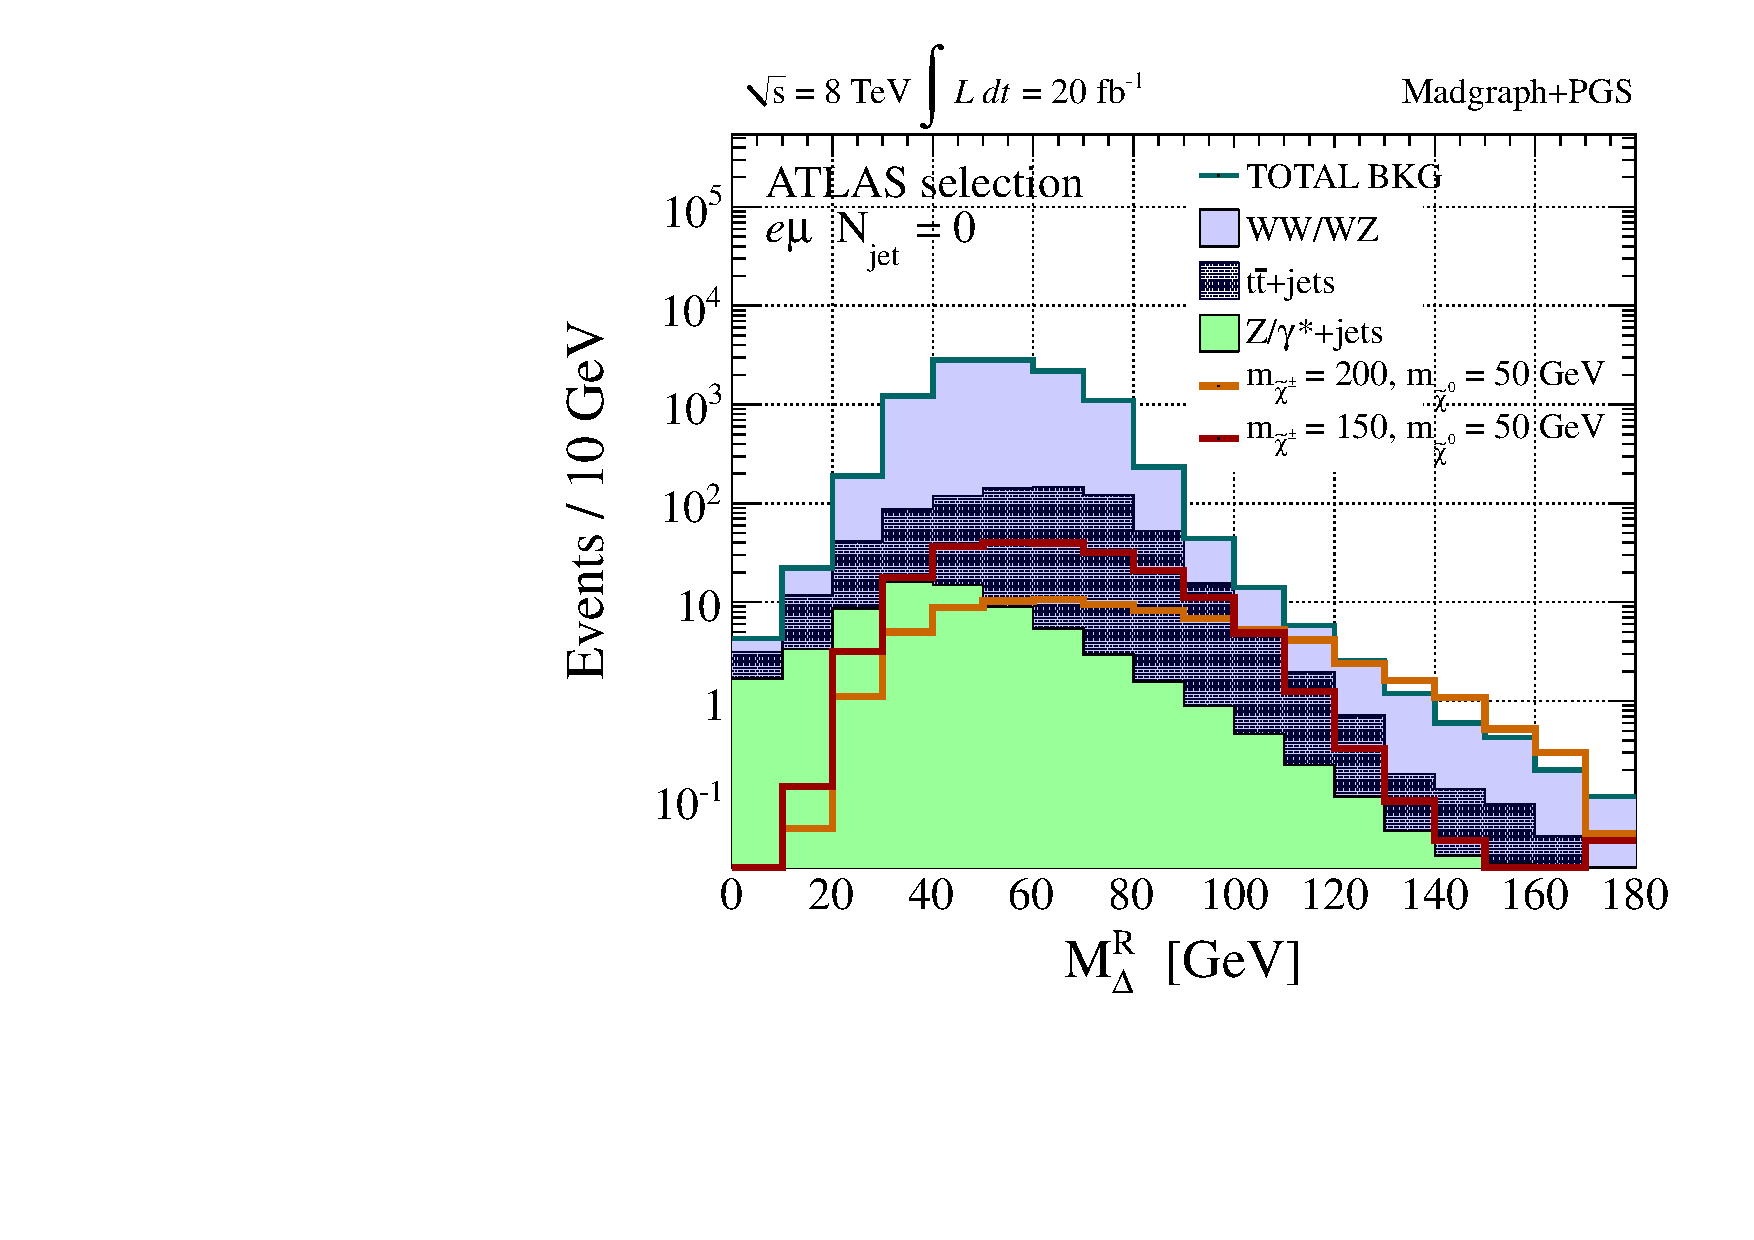
\includegraphics[width=0.35\columnwidth]{fig/sectionIV/PDF_chargino_ATLAS_Mdelta_OF_Njet0.pdf}
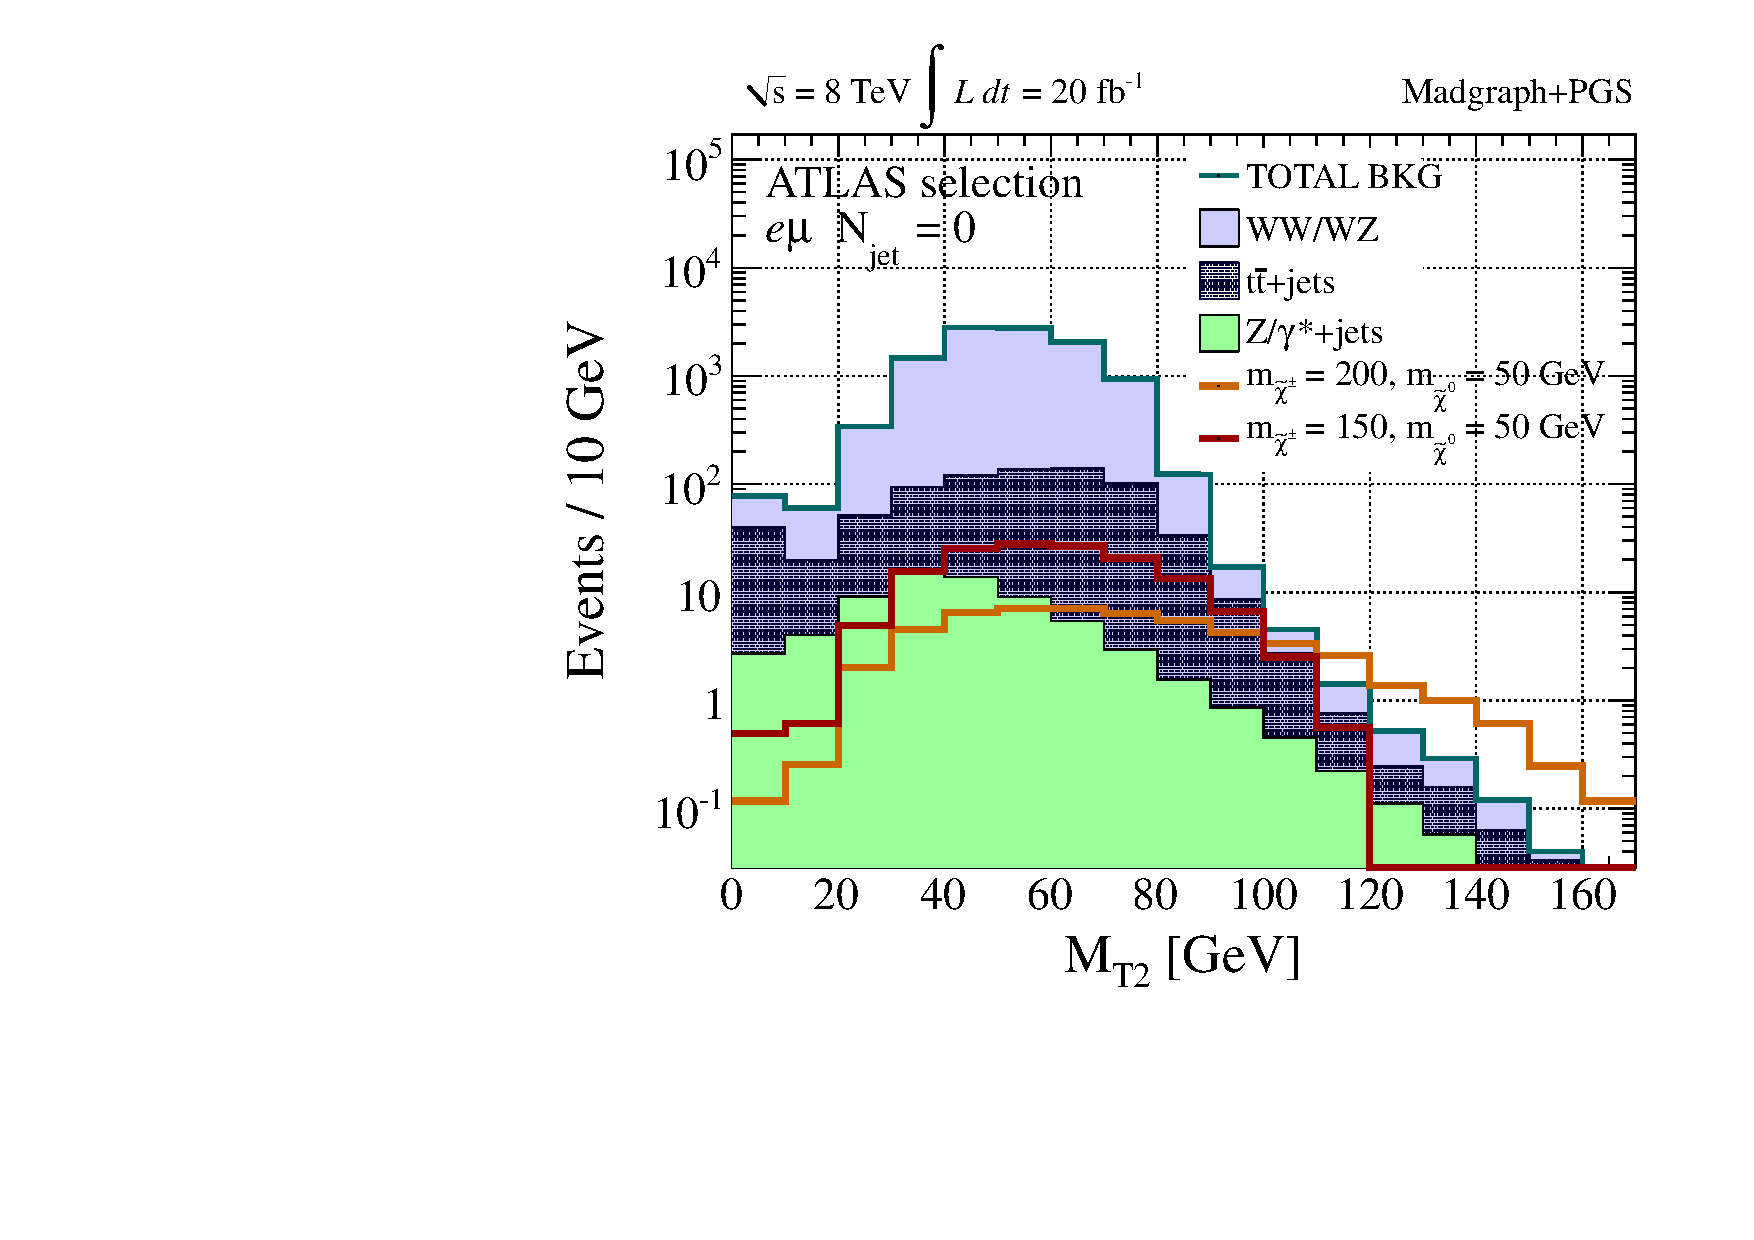
\includegraphics[width=0.35\columnwidth]{fig/sectionIV/PDF_chargino_ATLAS_MT2_OF_Njet0.pdf}
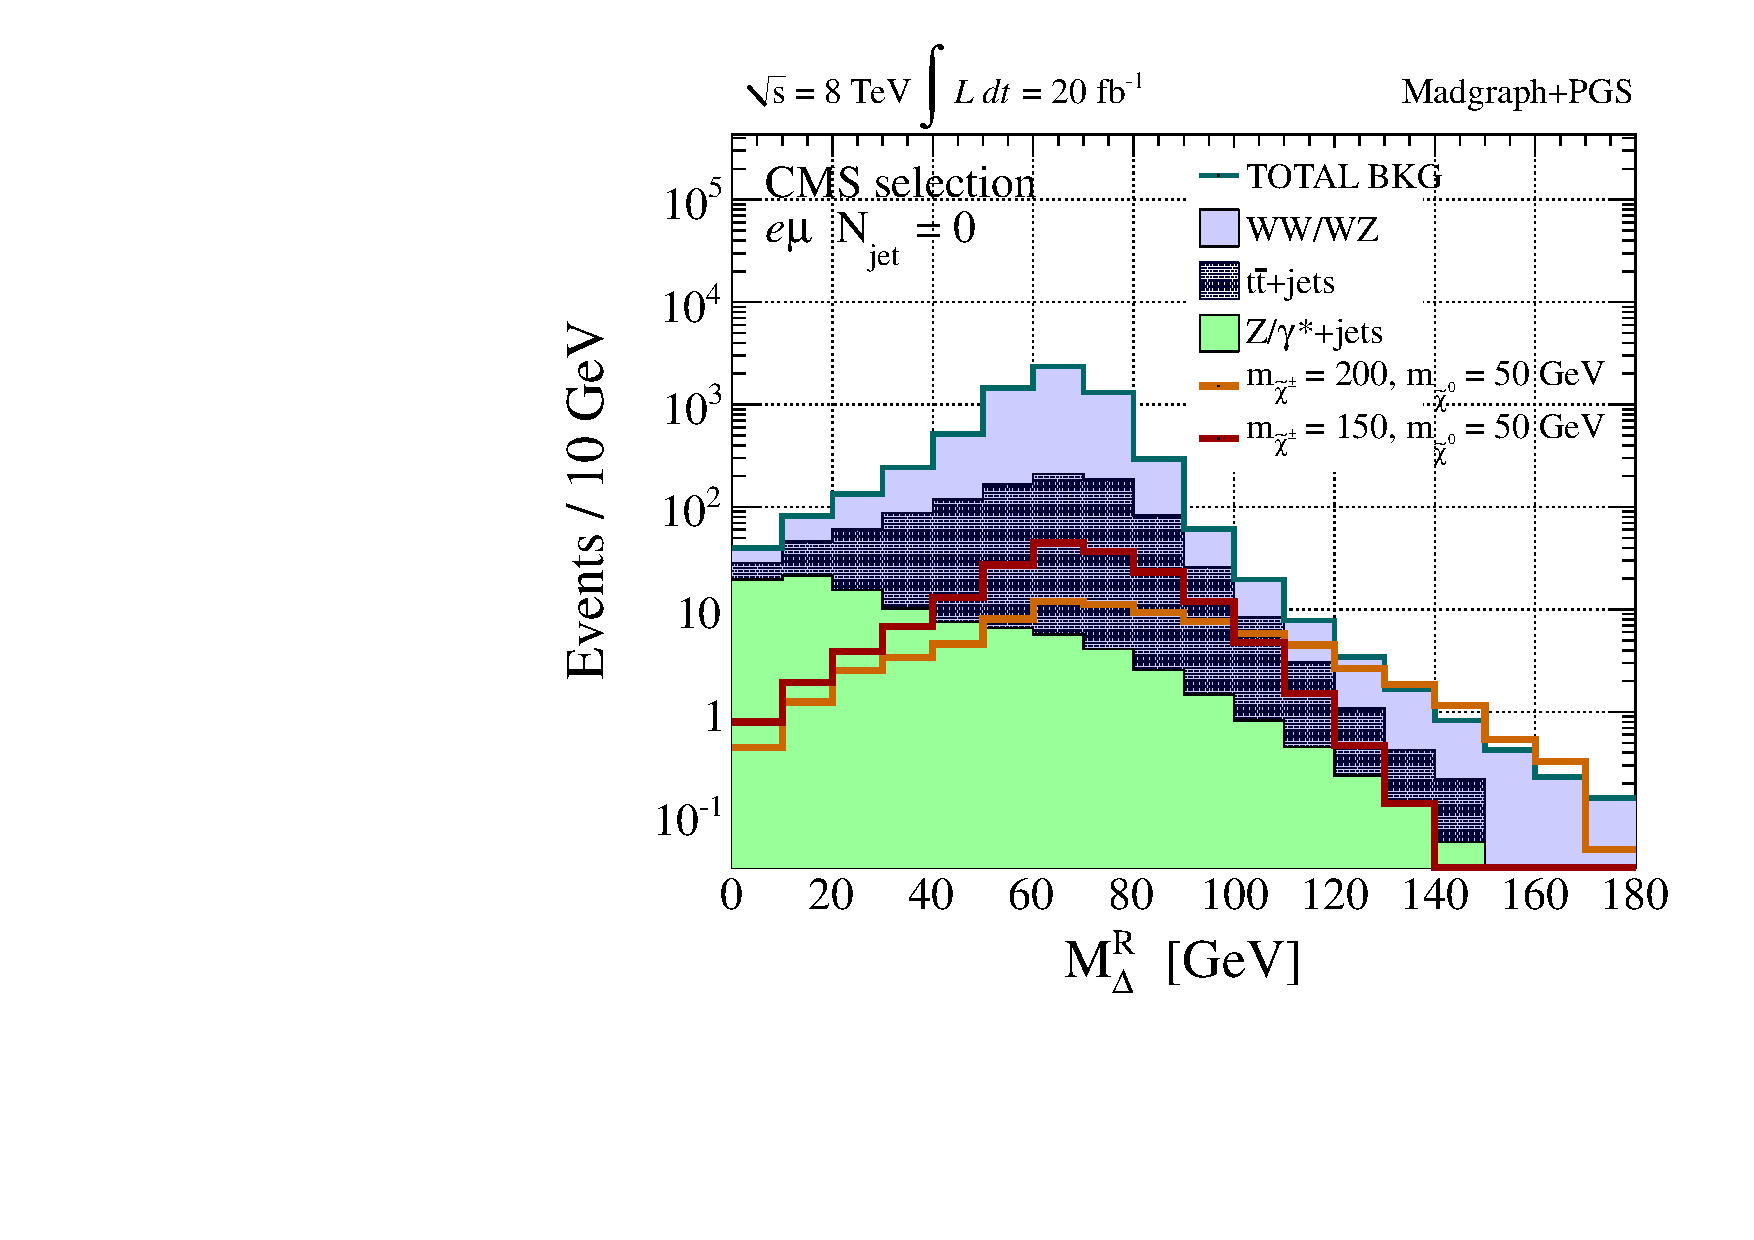
\includegraphics[width=0.35\columnwidth]{fig/sectionIV/PDF_chargino_CMS_Mdelta_OF_Njet0.pdf}
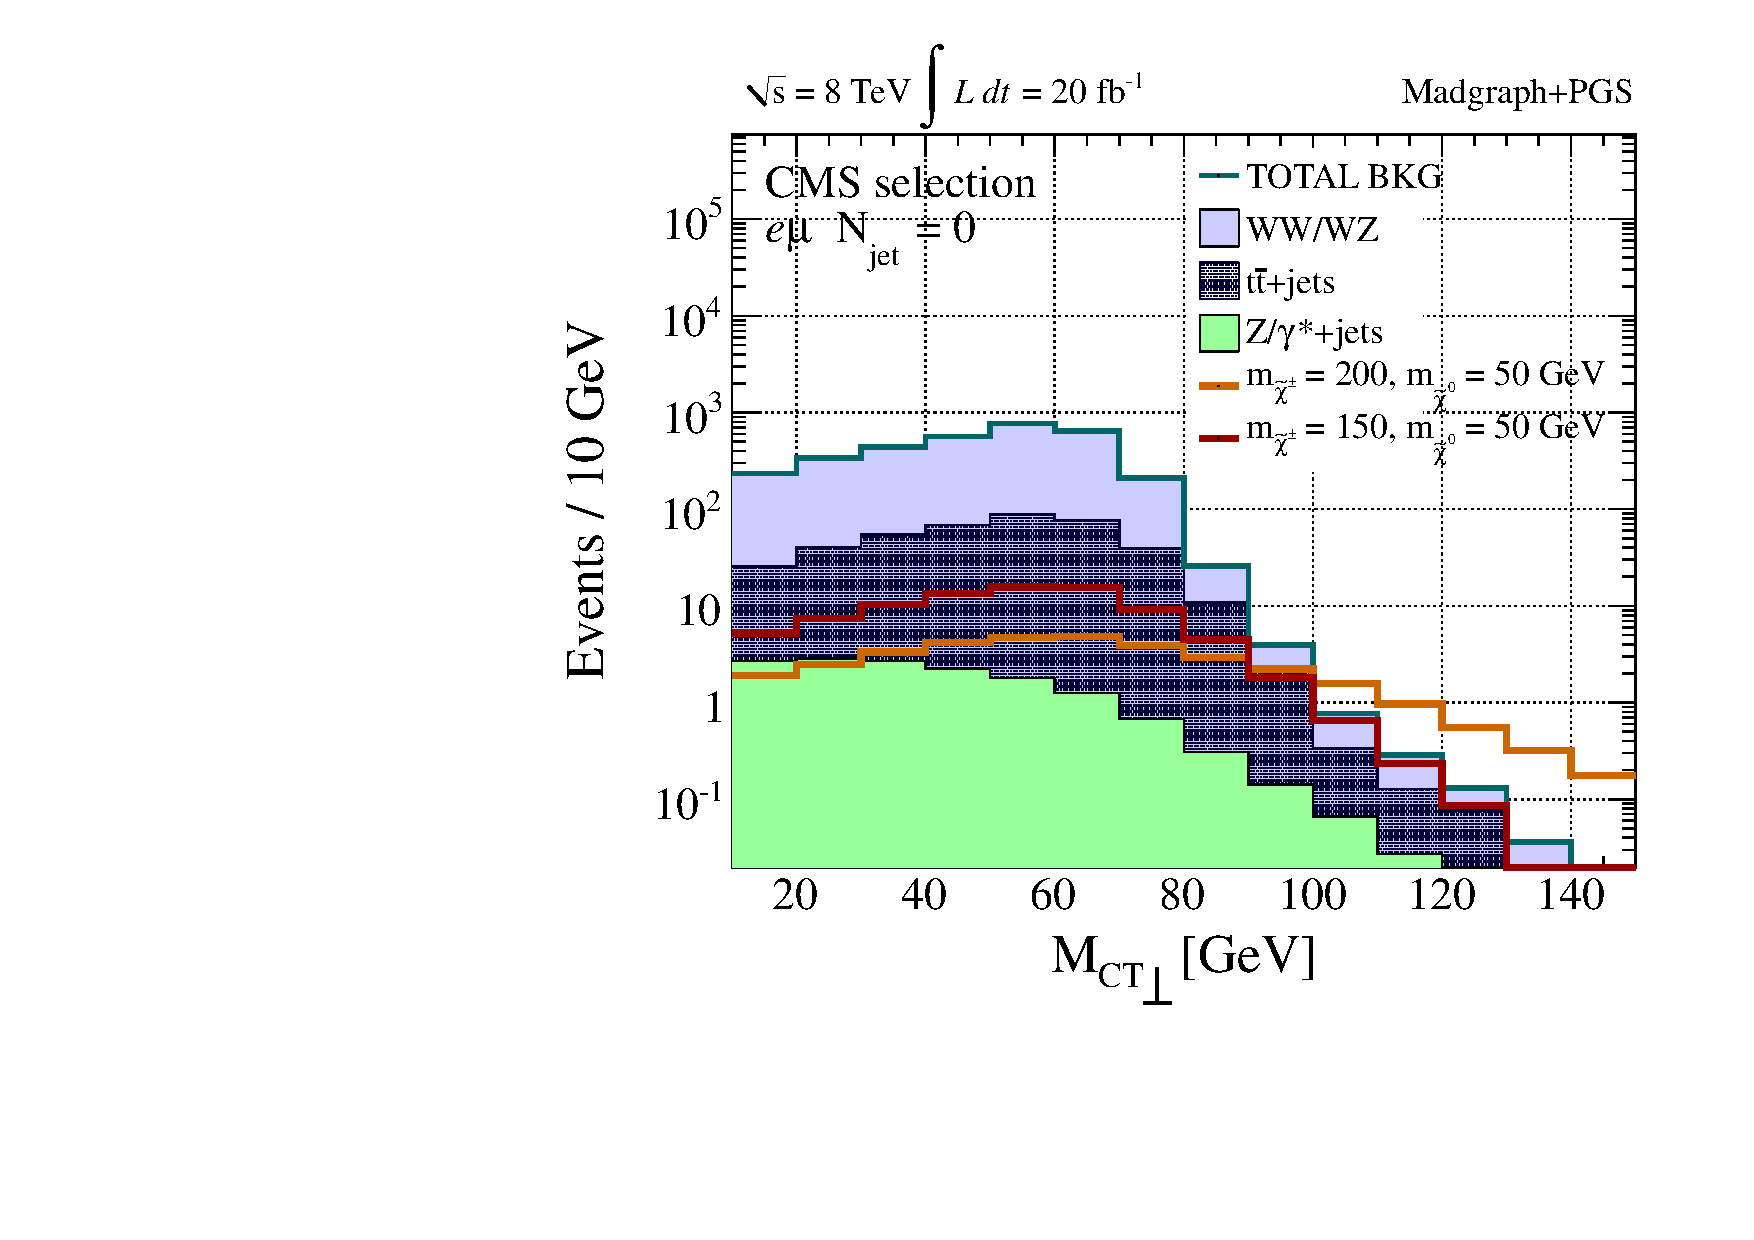
\includegraphics[width=0.35\columnwidth]{fig/sectionIV/PDF_chargino_CMS_MCTperp_OF_Njet0.pdf}
\caption{Expected background yields in the $e\mu$, $N_{jet} = 0$ final state passing the CMS or ATLAS selections, normalized to 20 fb$^{-1}$ of data. Top left: $M_{\Delta}^{R}$ with the ATLAS selection applied. Sample di-chargino signals are included with ($m_{\tilde{\chi}_{1}^{\pm}}= 200$,~$m_{\tilde{\chi}_{1}^0} = 50$) and ($m_{\tilde{\chi}_{1}^{\pm}} = 150$,~$m_{\tilde{\chi}_{1}^0} = 50$)~GeV.Top right: $M_{T2}$ with ATLAS selection. Bottom left: $M_{\Delta}^{R}$ with CMS selection. Bottom right: $M_{CT\perp}$ with CMS selection. \label{fig:EMUPDF}}
\end{figure}

In addition to one dimensional shape analyses using the variables $M_{\Delta}^{R}$, $M_{CT\perp}$, $M_{T2}$ we also consider a three-dimensional analysis based on $M_{\Delta}^{R}$, $|\cos\theta_{R+1}|$, and $\Delta\phi_{R}^{\beta}$. The two angular variables add complementary information to $M_{\Delta}^{R}$; $\Delta\phi^{\beta}$ introduces sensitivity to the ratio of neutralino and parent sparticle masses while $|\cos\theta_{R+1}|$ helps further resolve the scale $M_{\Delta}$ of a particular sample while also adding discrimination against $WW$ and $t\bar{t}$ using spin correlations (or lack thereof). Both of these angular variables are also useful in rejecting remaining Drell-Yan background events. 

The three dimensional $M_{\Delta}^{R} \times \Delta\phi_{R}^{\beta} \times |\cos\theta_{R+1}|$ analysis uses the razor selection described in the previous section, and represents each of the kinematic discriminants as binned histograms. For both signal and background events we find that the variable $\Delta\phi_{R}^{\beta}$ has only weak correlations with the other two variables. We neglect any residual correlations such that $\Delta\phi_{R}^{\beta}$ distributions are modeled as a one dimensional histogram with five equal-width bins ranging from between zero and $\pi$. Examples of expected event yields for SM backgrounds and representative signal models are shown in Figure~\ref{fig:DPHIPDF}.

\begin{figure}[ht]
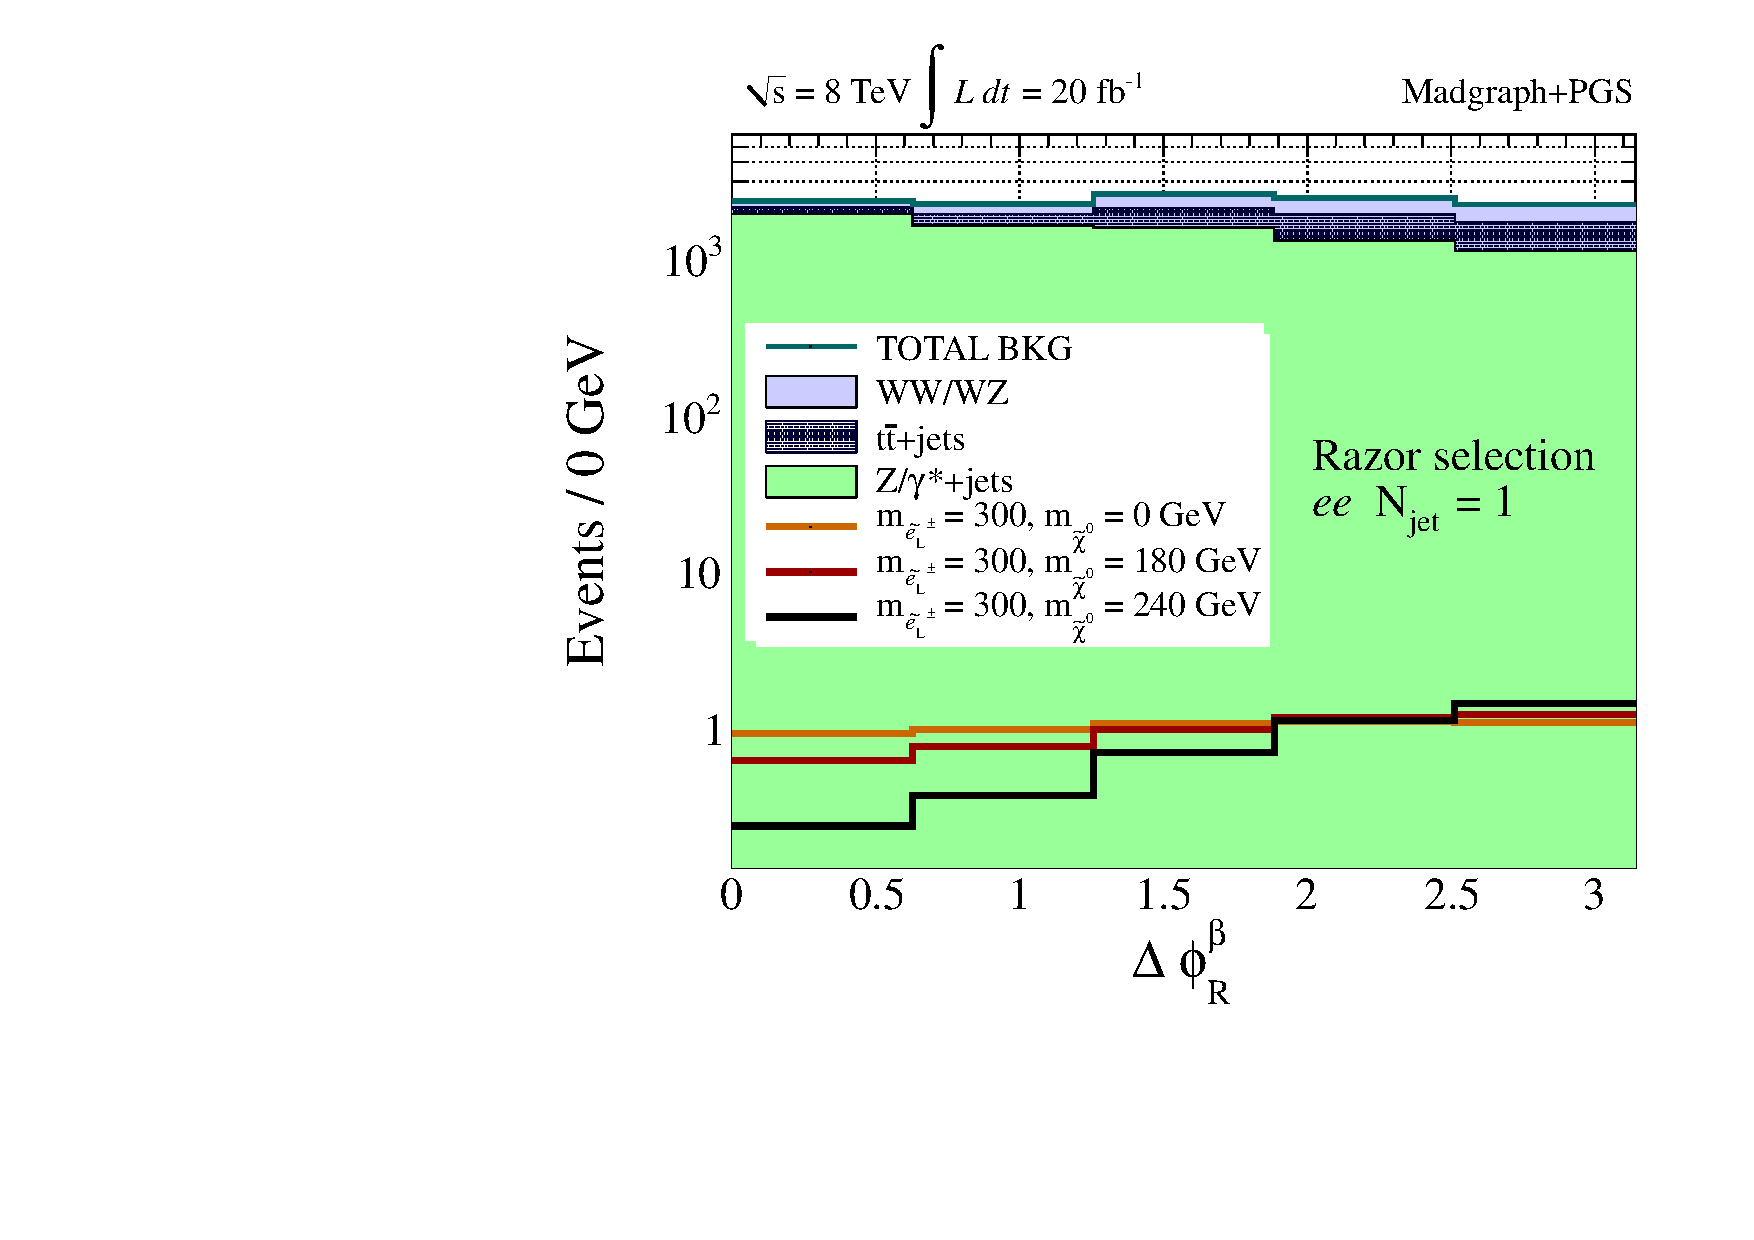
\includegraphics[width=0.35\columnwidth]{fig/sectionIV/PDF_selectronL_Razor_DPHI_ee_Njet1.pdf}
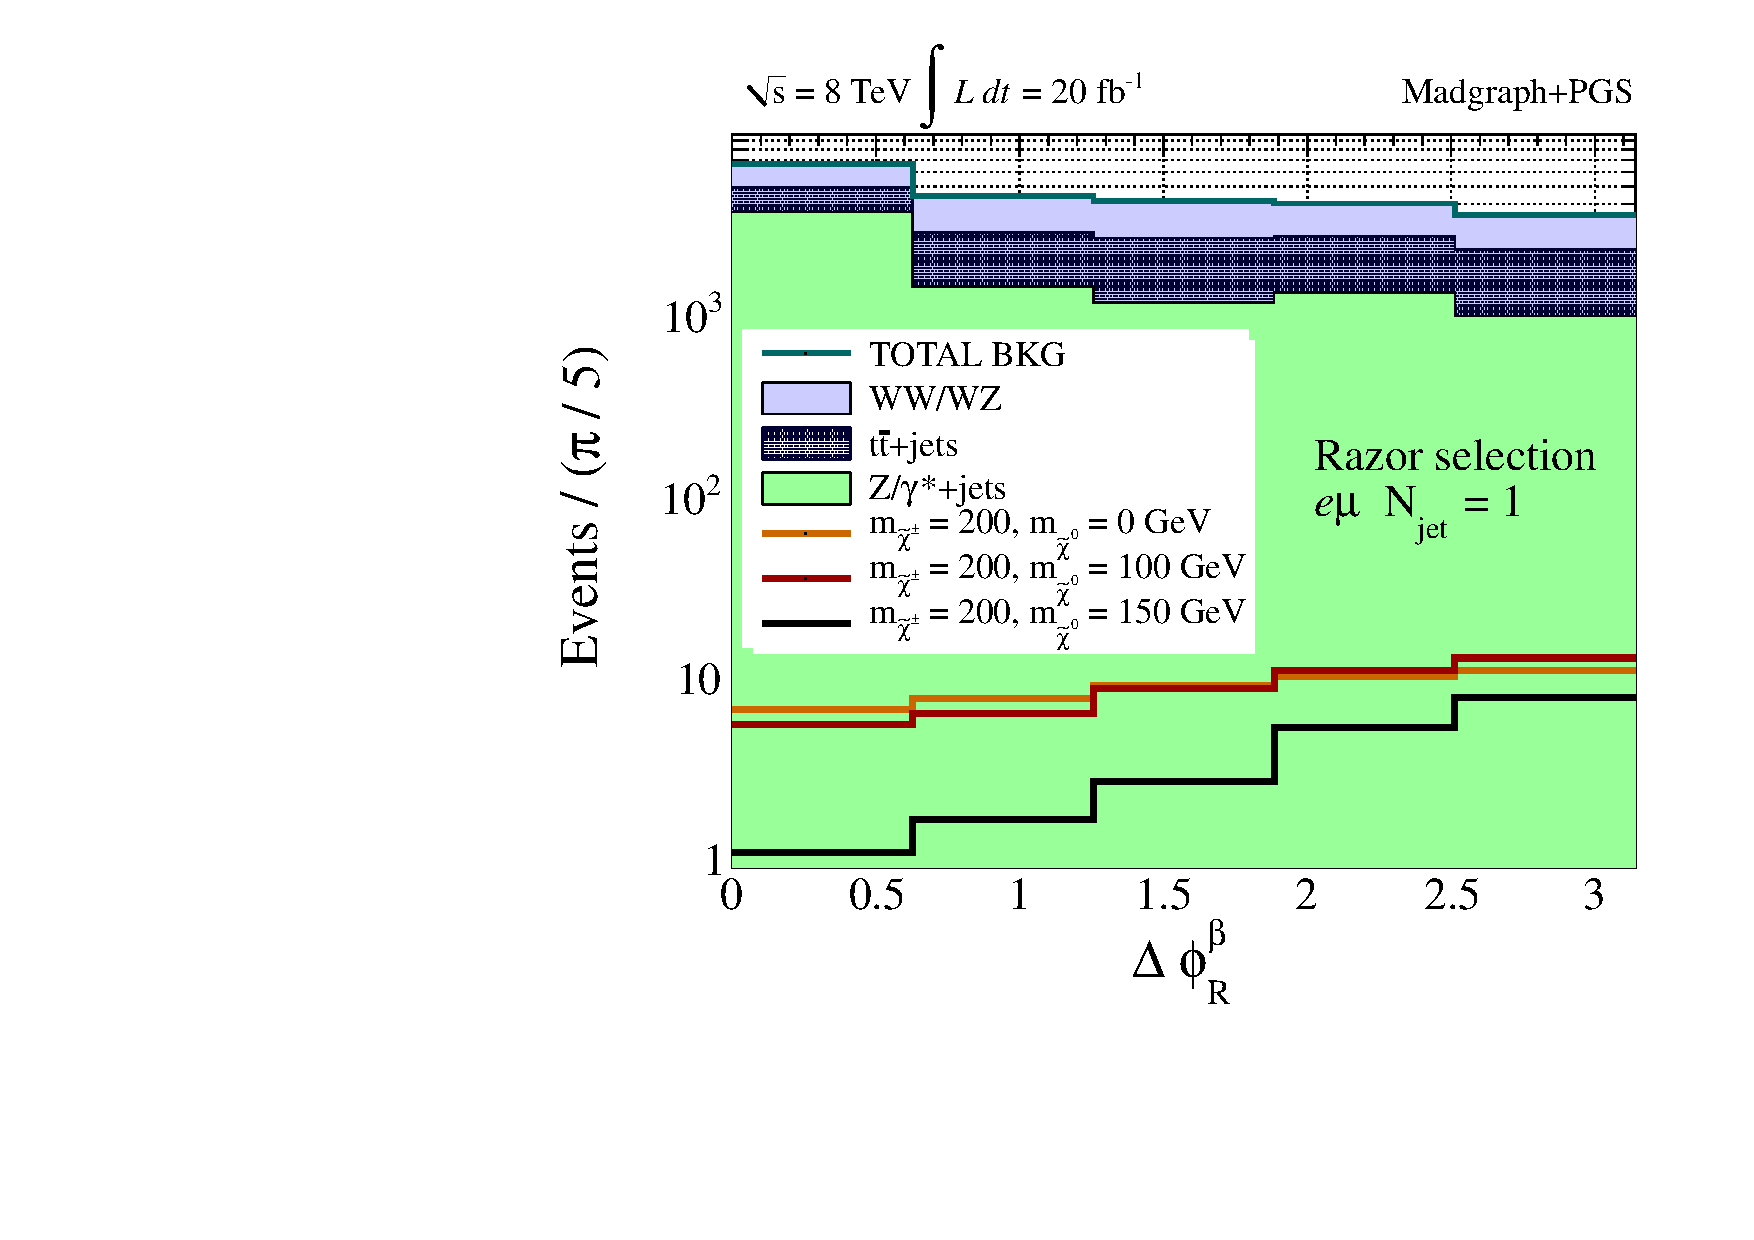
\includegraphics[width=0.35\columnwidth]{fig/sectionIV/PDF_chargino_Razor_DPHI_OF_Njet1.pdf}
\caption{Expected background yields in the $N_{jet} = 0$ final state passing the razor selection for $\Delta\phi_{R}^{\beta}$, normalized to 20 fb$^{-1}$ of data. Left: $ee$ final state including sample left-handed di-selectron signals with $m_{\tilde{\ell}} = 300$~GeV and varying neutralino masses. Right: $e\mu$ final state including sample di-chargino signals with $m_{\tilde{\chi}^{\pm}} = 200$~GeV and varying neutralino masses. \label{fig:DPHIPDF}}
\end{figure}

Strong correlations between $M_{\Delta}^{R}$ and $|\cos\theta_{R+1}|$ mean that these two variables cannot be factorized into one dimensional histograms. Rather, the two variables are modeled as two dimensional histograms with 10 GeV bins ranging from zero to 500 GeV for $M_{\Delta}^{R}$ (as for the one dimensional analysis) and 5 bins between zero and one for $|\cos\theta_{R+1}|$. The expected event yields for the sum of the SM backgrounds and sample signal models in this two dimensional binning are shown in Fig.~\ref{fig:COSTHETAPDF}

\begin{figure}[ht]
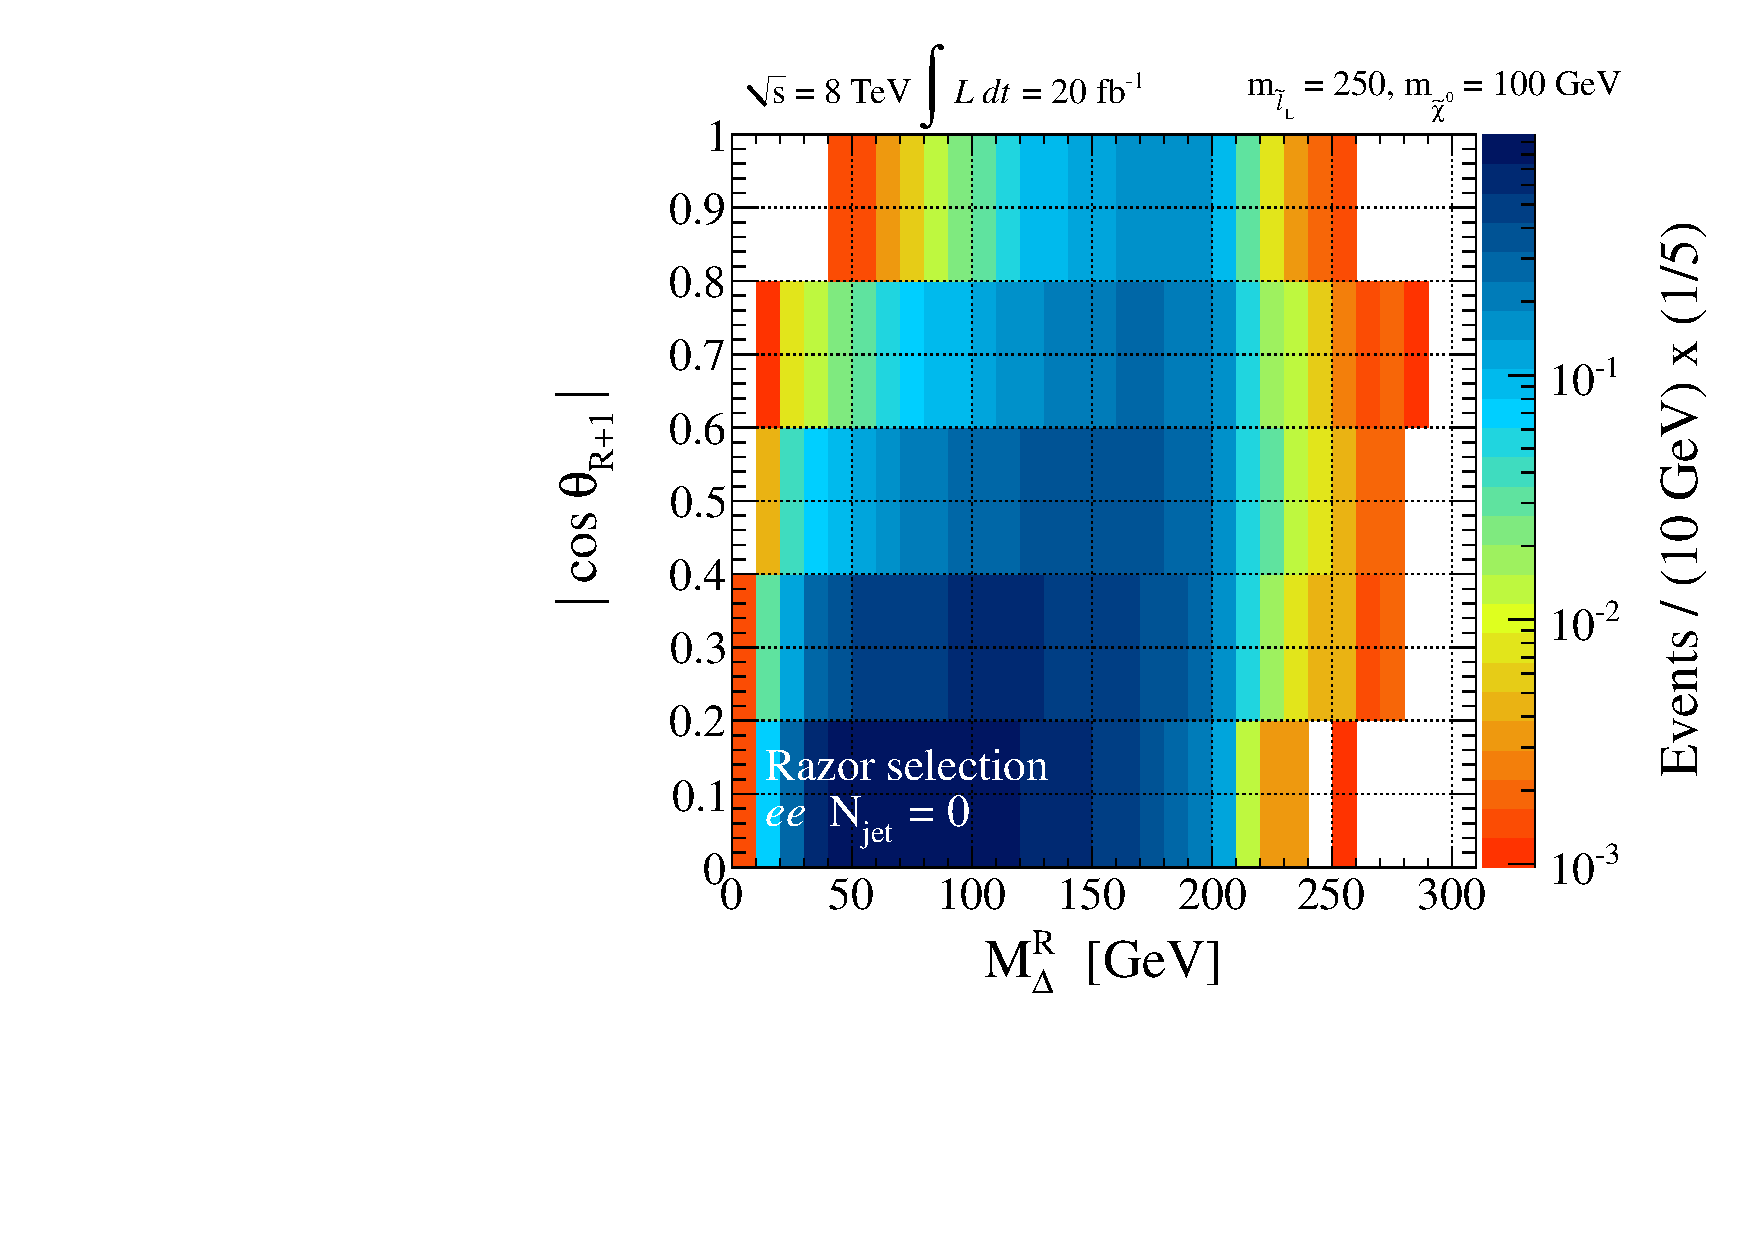
\includegraphics[width=0.35\columnwidth]{fig/sectionIV/PDF_2D_ee_selectron.pdf}
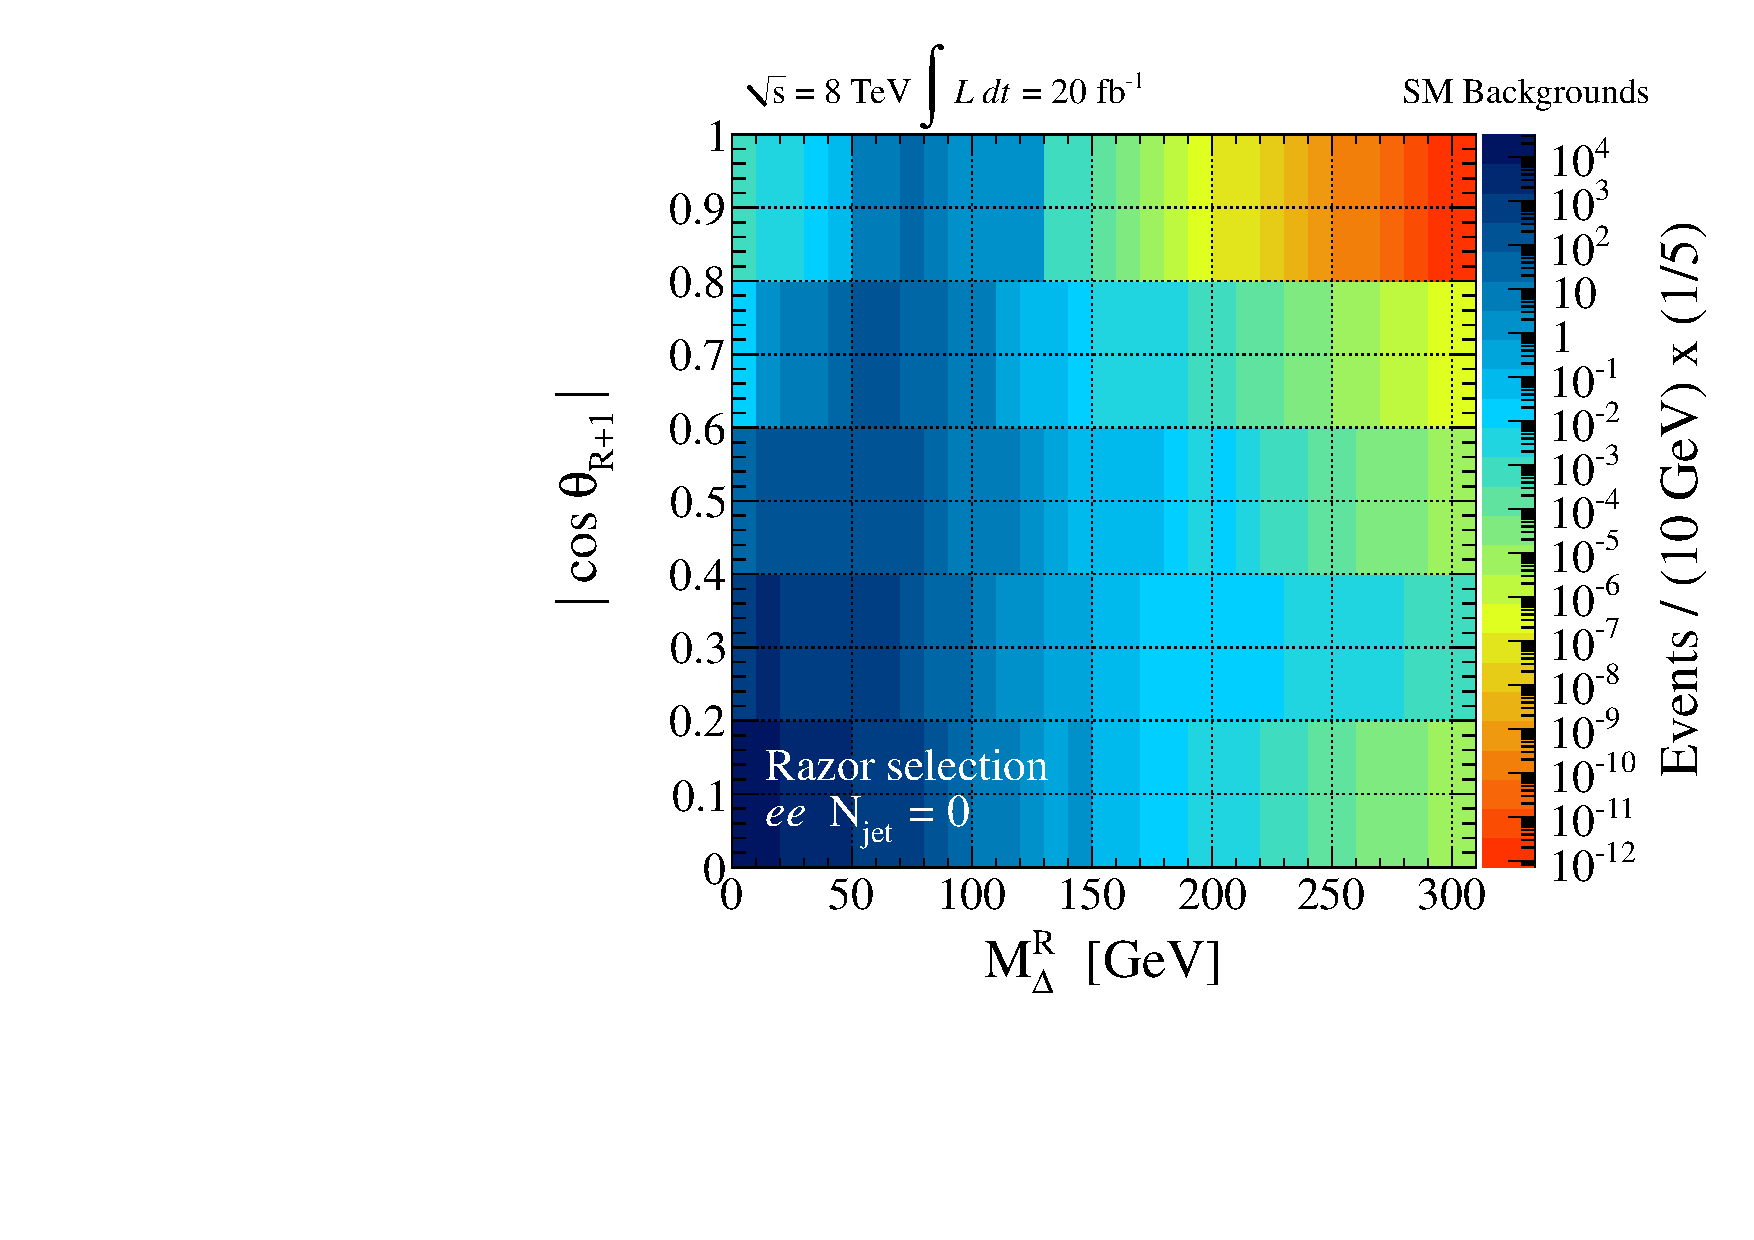
\includegraphics[width=0.35\columnwidth]{fig/sectionIV/PDF_2D_ee_BKG.pdf}
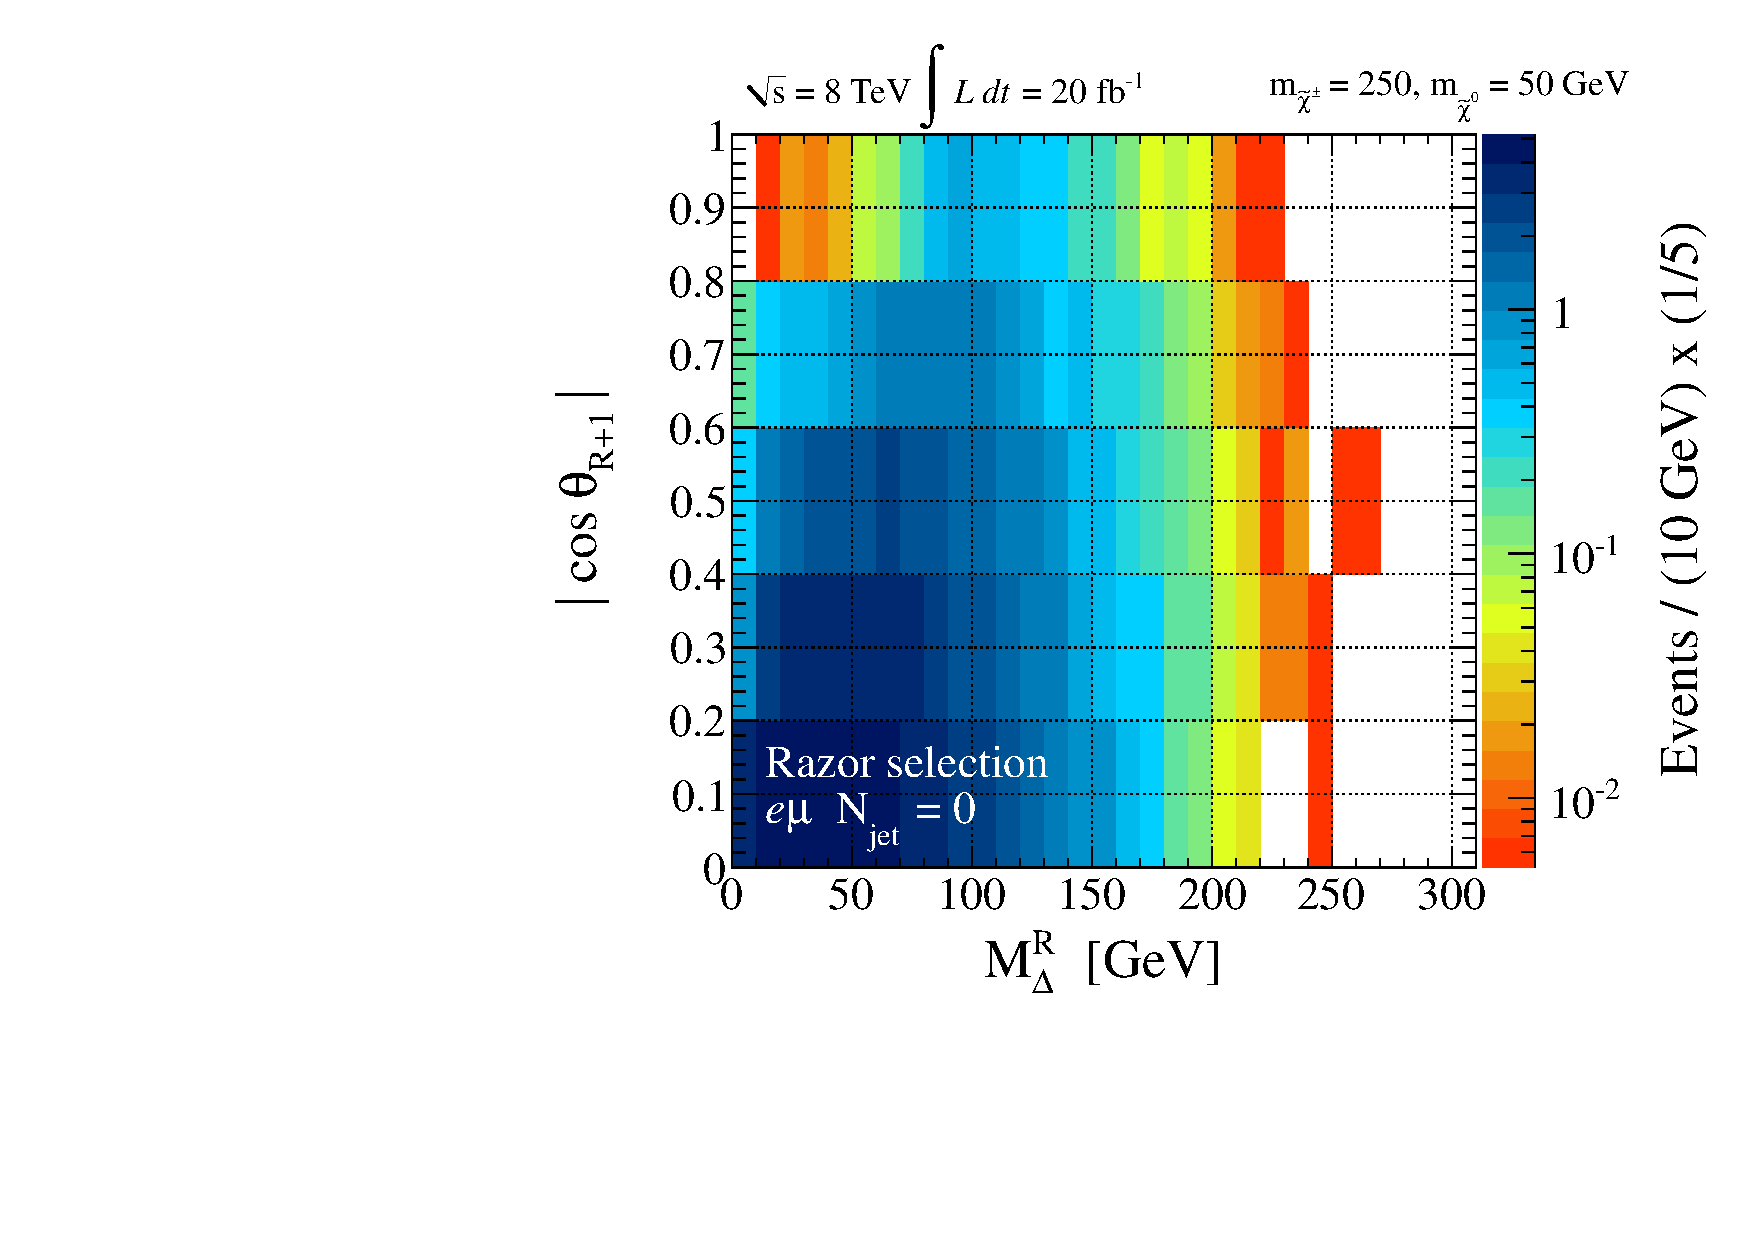
\includegraphics[width=0.35\columnwidth]{fig/sectionIV/PDF_2D_emu_chargino.pdf}
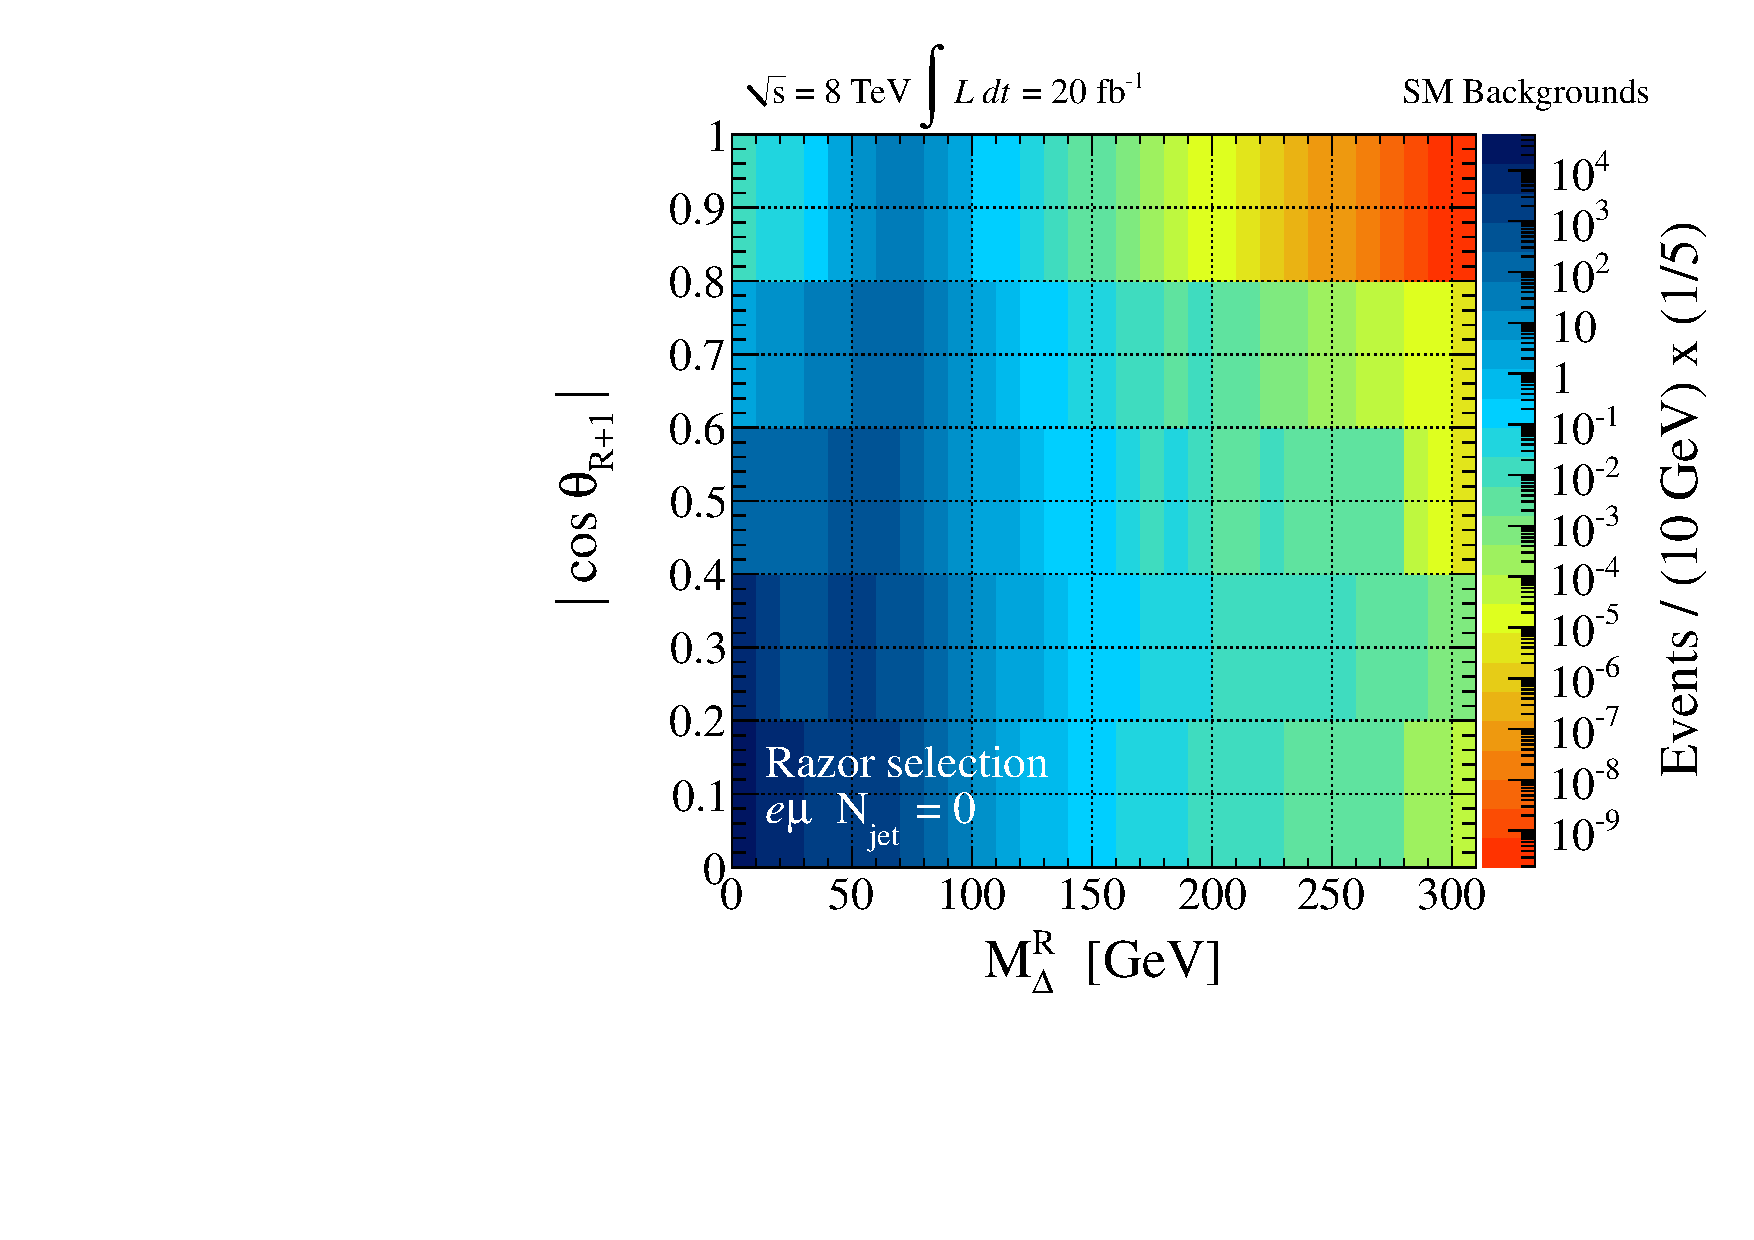
\includegraphics[width=0.35\columnwidth]{fig/sectionIV/PDF_2D_emu_BKG.pdf}
\caption{Expected background yields in $M_{\Delta}^{R} \times |\cos\theta_{R+1}|$ plane, normalized to 20 fb$^{-1}$ of data. Top: Expected event yields for the $ee$ final state with $N_{jet} = 0$ and the Razor selection applied. Bottom: Analogous figures for the $e\mu$ final state. Left: Kinematic distributions for sample signal models including di-selectron production with ($m_{\tilde{\ell}_L}=250$, $m_{\tilde{\chi}^{0}_{1}}=100$) GeV (top left) and di-chargino production with ($m_{\tilde{\chi}^{\pm}_1}=250$, $m_{\tilde{\chi}^{0}_{1}}=50$)  GeV (bottom left). Right: Total of expected SM background yields. \label{fig:COSTHETAPDF}}
\end{figure}

\subsection{Fit to toy data and statistical analysis}

For each dataset a fit is performed over all final state categories and bins of the kinematic discriminants simultaneously, measuring the yields of different background contributions. The fit proceeds by maximizing the binned likelihood for the dataset being examined, which can be written as
\begin{equation}
\log {\cal L} = \sum_{i} \log \left( \frac{ b_{i}^{n_{i}}e^{-b_{i}} }{n_{i}!} \right) ~,
\label{eq:simple}
\end{equation}
where $i$ runs over all of the bins and $b_{i}$ and $n_{i}$ are the expected and observed number of events in that bin, respectively. For each toy analysis fit the likelihood is maximized over the yields of each of the backgrounds, subject to constraints between bins so that the full likelihood can be written
\begin{equation}
\log {\cal L}[b_{0},\cdots,b_{N_{p}}] = \sum_{c}\sum_{k} \left[ n_{ck} \log \left(\sum_p b_{p} \hat{b}_{pck}\right) - \sum_p b_{p} \hat{b}_{pck}\right] ~,
\label{eq:full}
\end{equation}
where bins are now indexed by category ($c$) and kinematic discriminant bin ($k$). The total expected number of events for a single process $p$ is $b_{p}$ while $\hat{b}_{pck}$ is the fraction of events from process $p$ expected to fall into bin $ck$, such that the number of expected events in a bin $i$ from Equation~\eqref{eq:simple}, $b_{i}$, has become $\sum_p b_{p} \hat{b}_{pck}$. While the total normalization of each process is independent from the others, the probability distribution function (pdf) of each process, $\hat{b}_{pck}$, provides constraints between different categories and bins of the kinematic discriminant.

Two fits are performed on each dataset, one corresponding to the background-only hypothesis and the other to the signal plus background hypothesis, where the signal corresponds to whichever model is being tested. The background only fit can be represented as
\begin{equation}
\log {\cal L}_{b} = \max_{b_{\mathrm{DB}},b_{t\bar{t}},b_{\mathrm{DY}}} {\cal L} [b_{\mathrm{DB}},b_{t\bar{t}},b_{\mathrm{DY}}]
\label{eq:Lb}
\end{equation}
where $b_{\mathrm{DB}}$, $b_{t\bar{t}}$, and $b_{\mathrm{DY}}$ represent the normalizations for di-boson, $t\bar{t}$ and Drell-Yan backgrounds, respectively. Similarly, the signal plus background fit maximizes the likelihood
\begin{equation}
\log {\cal L}_{s+b} = \max_{b_{\mathrm{DB}},b_{t\bar{t}},b_{\mathrm{DY}}} {\cal L} [b_{s} = \hat{N}_{S},b_{\mathrm{DB}},b_{t\bar{t}},b_{\mathrm{DY}}]
\label{eq:Lspb}
\end{equation}
which differs from $\log {\cal L}_{b}$ in Equation~\eqref{eq:Lb} by the addition of a signal contribution with total yield $b_{s}$. This yield is not floated in the fit; rather, it is fixed to the expected number of signal events for a given model, $\hat{N}_{S}$. The two maximized likelihoods, ${\cal L}_{b}$ and ${\cal L}_{s+b}$, are combined to form the test-statistic used to quantify the separation between the two hypotheses for a given model and dataset, the log-likelihood ratio $\lambda$
\begin{equation}
\lambda = \log \left( {\cal L}_{s+b} / {\cal L}_{b} \right)
\end{equation}

Systematic uncertainties are included in this procedure through marginalization. In this scheme, the kinematic discriminant pdf shapes and normalizations used in the likelihood evaluation remain fixed at their nominal values. During the toy dataset generation process these same shapes and normalizations are systematically varied according to expected uncertainties. We consider several sources and qualitative types of systematic uncertainties. A 10\% uncertainty is applied independently to each SM background process cross-section. The effect of this uncertainty is largely mitigated during the maximization of the likelihoods (where normalizations are floated). For backgrounds with multiple sub-contributions, like di-boson production, the relative sub-process yields are fixed in the likelihood evaluation resulting in an effective shape uncertainty. Each of the expected signal yields is also varied based on a calculation of the theoretical cross-section uncertainty. 

In addition to overall normalization uncertainties there are also a collection of variations which change the shape of background pdfs, both by varying the relative yields in different final state categories and by altering the shapes of the kinematic discriminants themselves. A 2\% uncertainty is assigned for the reconstruction and identification of each lepton, uncorrelated between lepton flavors.  This uncertainty is assumed to be correlated between different processes. Similarly, a 10\% uncertainty is assigned for the reconstruction and identification of each additional jet, effectively varying the relative yields between different jet multiplicity categories, independently for each process. This is meant to account for not only experimental effects relevant to jet counting, such as jet energy scale (JES) and resolution but also theoretical uncertainties in the production of strong emissions. To introduce uncertainty in the shape of kinematic discriminants we propagate the effects of potential JES uncertainties to the $E_{T}^\text{miss}$ and kinematic variable calculation. For each simulated event all of the reconstructed jets, without a $p_{T}$ threshold, are varied in $p_{T}$ either up or down by 10\%. The different between the original and new jet momenta is added vectorially to the $\vec{E}_{T}^\text{miss}$ and the kinematic variables of interest (for both selection requirements and kinematic discriminants) are recalculated using both the up and down variations separately. Each of the datasets corresponding to these variations are used to re-derive pdfs for the kinematic variables of interest such that the pdf shape for a given toy experiment is taken from a linear combination of the up, down and nominal templates. 

For each signal model a series of toy pseudo-experiments are performed. For each pseudo-experiment, the parameters describing each of the systemic uncertainties are varied, yielding a new set of pdfs and normalizations for each process. These are then used to generate two toy data samples for the pseudo-experiment, with one set including the expected contribution of the signal in the data sample and another without the signal. Each dataset in the pseudo-experiment is then fit to each of the hypotheses (signal or no signal), yielding the maximized likelihoods ${\cal L}_{b}$ and ${\cal L}_{s+b}$ and the test-statistic $\lambda$. Repeating this procedure for many toys allows us to estimate the expected distribution of $\lambda$ in the case that there is only background in the data sample, $P(\lambda | b~\mathrm{only})$ and when there is also signal, $P(\lambda | s+b)$. Example distributions of $\lambda$ for pseudo-experiments corresponding to representative signal models and analyses are shown in Figure~\ref{fig:bells}.

\begin{figure}[ht]
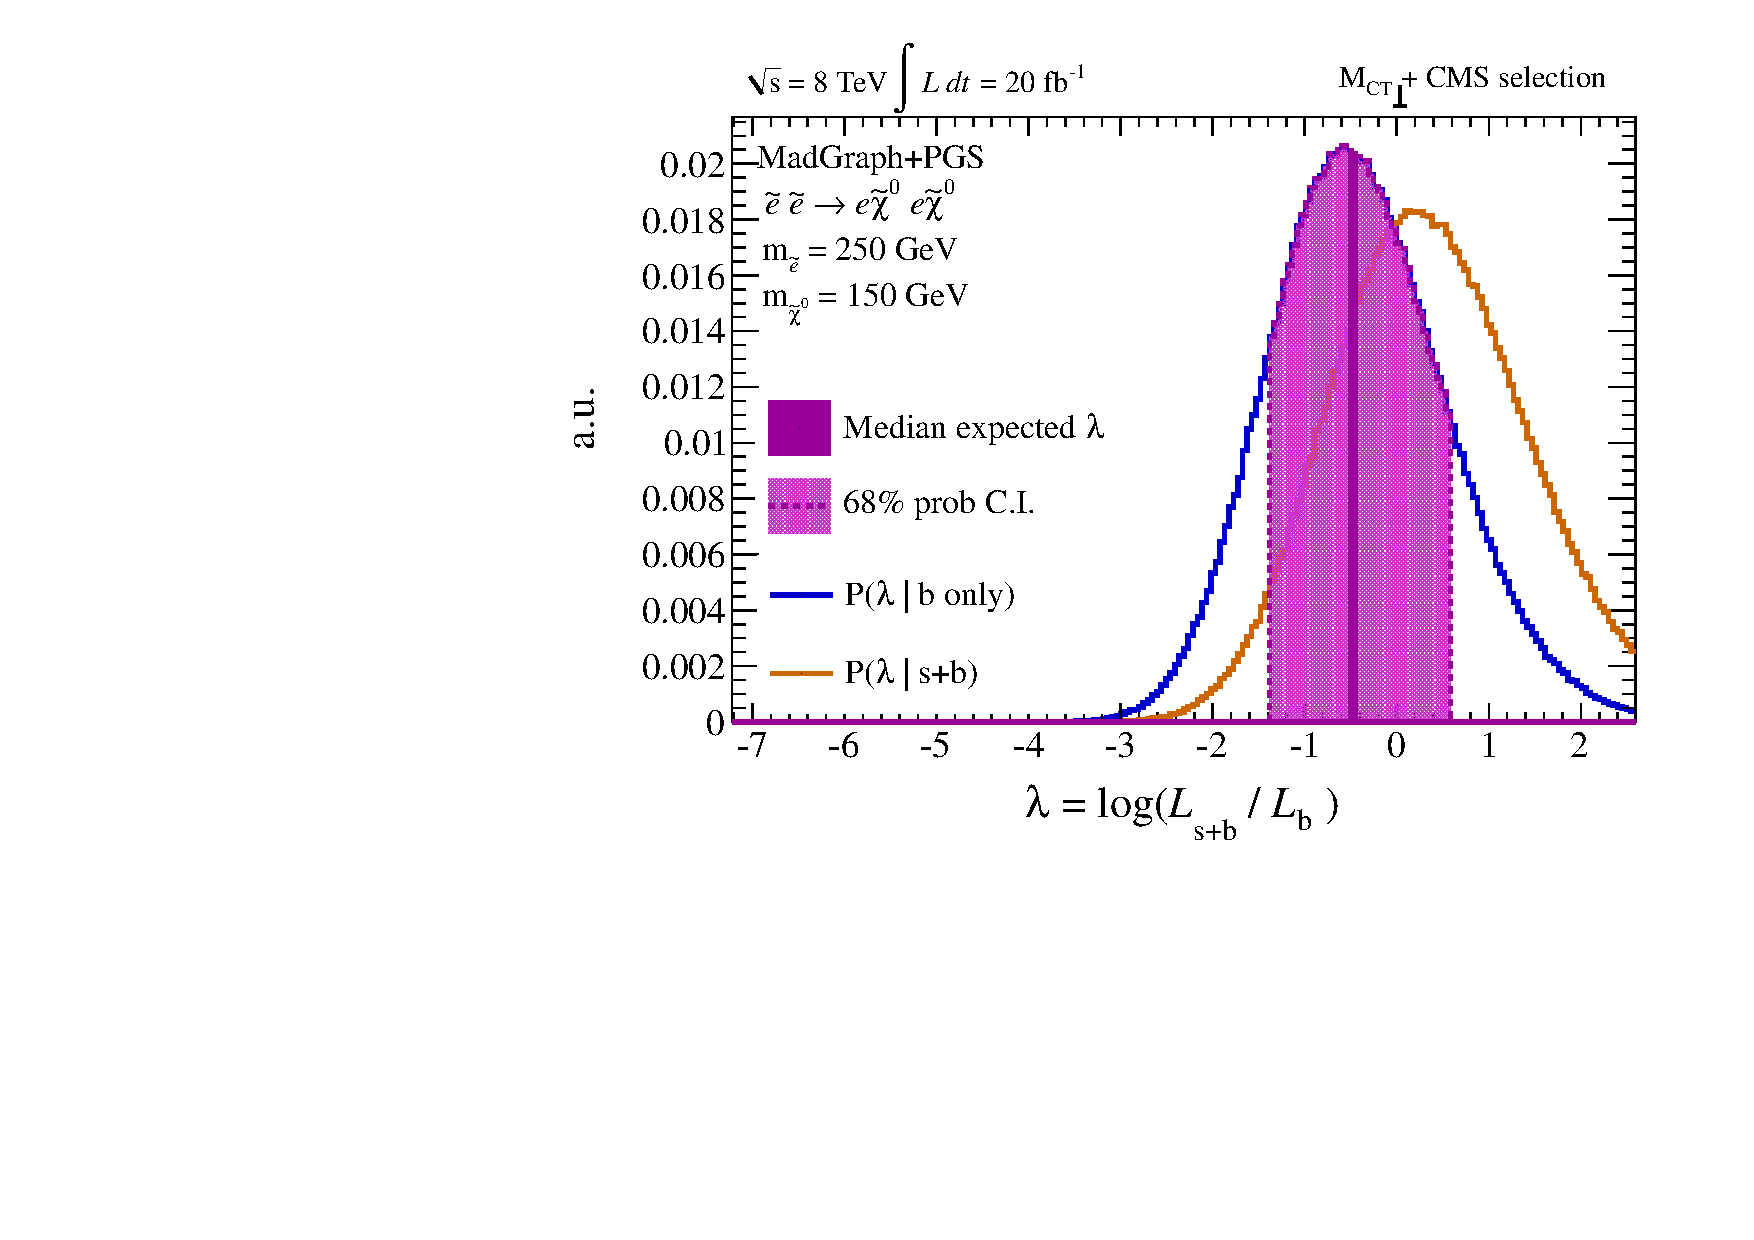
\includegraphics[width=0.35\columnwidth]{fig/sectionIV/BELLS1D_exp_selectron250_150_ANA2.pdf}
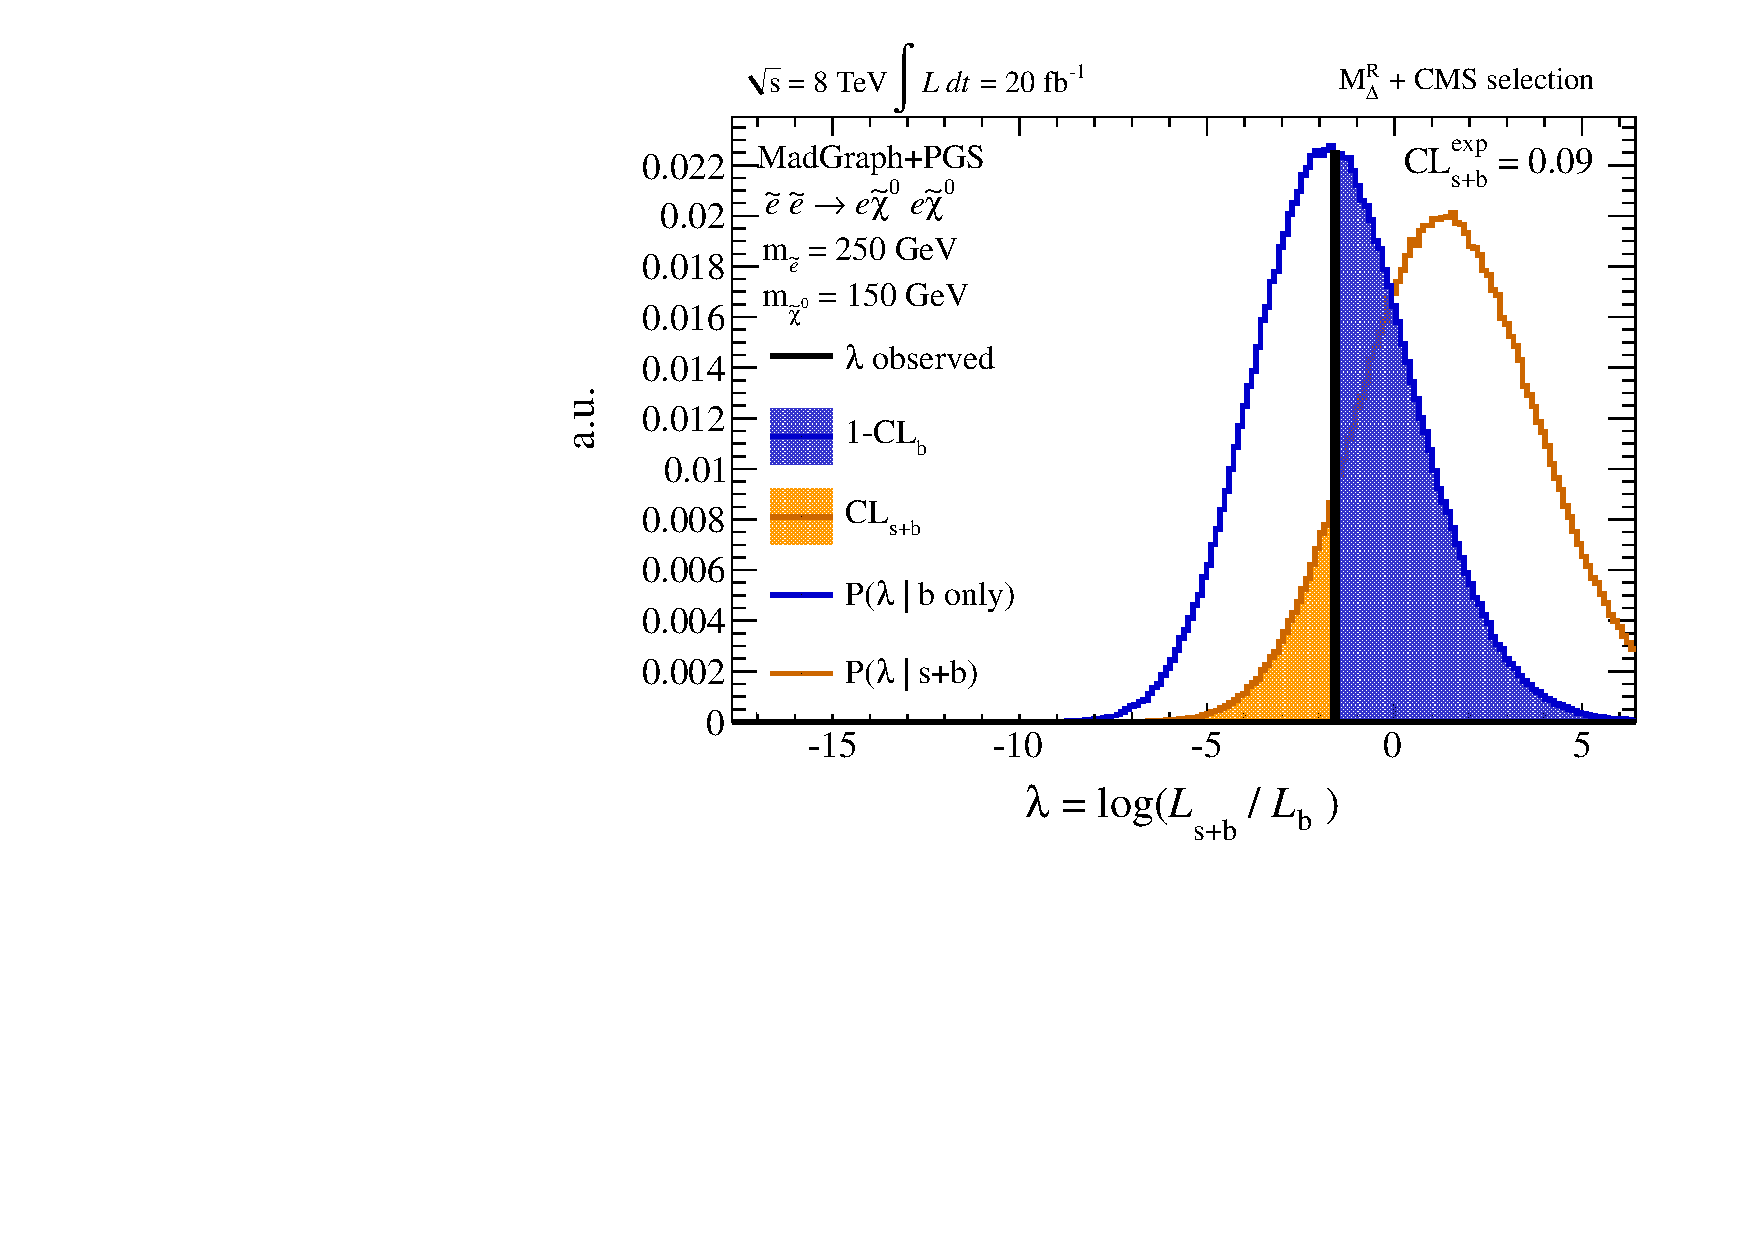
\includegraphics[width=0.35\columnwidth]{fig/sectionIV/BELLS1D_obs_selectron250_150_ANA0.pdf}
\caption{Distributions of $\lambda$, assuming both signal and background-only scenarios. Left: Test-statistic distributions for the one-dimensional $M_{CT\perp}$ analysis searching for di-selectron production with ($m_{\tilde{\ell}_L}=250$~GeV, $m_{\tilde{\chi}^{0}_{1}}=150$~GeV). Right: $\lambda$ distributions for the one-dimensional $M_{\Delta}^{R}$ analysis, using the same mass point. \label{fig:bells}}
\end{figure}

The expected sensitivity of a given search is calculated from these test-statistic distributions. In order evaluate the probability of observing a given $\lambda$ value in an experiment ($\lambda^{\mathrm{exp}}$) the expected pdfs of $\lambda$ are used to calculate the quantities CL$_{b}$ an CL$_{s+b}$ as
\begin{eqnarray}
\mathrm{CL}_{b} = \int_{-\infty}^{\lambda^{\mathrm{exp}}} P(\lambda | b~\mathrm{only})~, \nonumber \\
\mathrm{CL}_{s+b} = \int_{-\infty}^{\lambda^{\mathrm{exp}}} P(\lambda | s+b)~.
\end{eqnarray}
CL$_{b}$ is the probability of observing a $\lambda$ at least as background-like as $\lambda^{\mathrm{exp}}$ assuming that there is no signal contribution, while CL$_{s+b}$ is the same probability assuming there is signal injected. In order to quantify the expected sensitivity of an analysis we choose $\lambda^{\mathrm{exp}}$ to be the median expected $\lambda$ assuming it is distributed as $P(\lambda | b~\mathrm{only})$. The resulting CL$_{s+b}$ is then the median expected $p$-value for a given signal hypothesis, with lower values indicating that the model would be excluded at higher significance. These expected $p$-values are converted into a number of $\sigma$, corresponding to a normally distributed set of outcomes, as
\begin{equation}
N~\sigma = \sqrt{2} ~\mathrm{erf}^{-1} (\mathrm{CL}_{s+b})~.
\end{equation}
A particular model is expected to be excluded at 95\% confidence level (C.L.) if the median expected CL$_{s+b}$ is less than 0.05, and $N \sigma \ge 1.96$. The CMS and ATLAS experiments choose to quote results in the context of the CL$_{s}$ convention~\cite{Junk:1999kv,Read:2002hq}, where CL$_{s}$ = CL$_{s+b}$/CL$_b$. For median expectations, CL$_b$ is exactly 1/2, implying that a CL$_{s} \le 0.05$ threshold for excluding a given hypothesis corresponds to a 97.5\% C.L. exclusion, or $N \sigma \ge 2.24$. 

The expected exclusions for di-slepton signals at 97.5\% C.L. for analyses performed with 20 fb$^{-1}$ of integrated luminosity at $\sqrt{s} = 8$~TeV, evaluated using this statistical approach, are shown in Figure~\ref{fig:CLs}. Comparing the excluded models from these toy analyses with those from the actual CMS \cite{CMS-PAS-SUS-13-006} and ATLAS \cite{ATLAS-CONF-2013-049} searches we observe that the results are in reasonable agreement. The expectations from toy experiments tend to be more optimistic than the actual experimental results, which is expected given that kinematic discriminants are being used in a shape analysis and deficiencies in detector simulation likely correspond to underestimated resolution effects, particularly for $E_{T}^\text{miss}$. Regardless, this toy analysis framework allows for a quantitative comparison of different kinematic discriminants in the context of an analysis with realistic experimental effects at least partially accounted for.

\begin{figure}[ht]
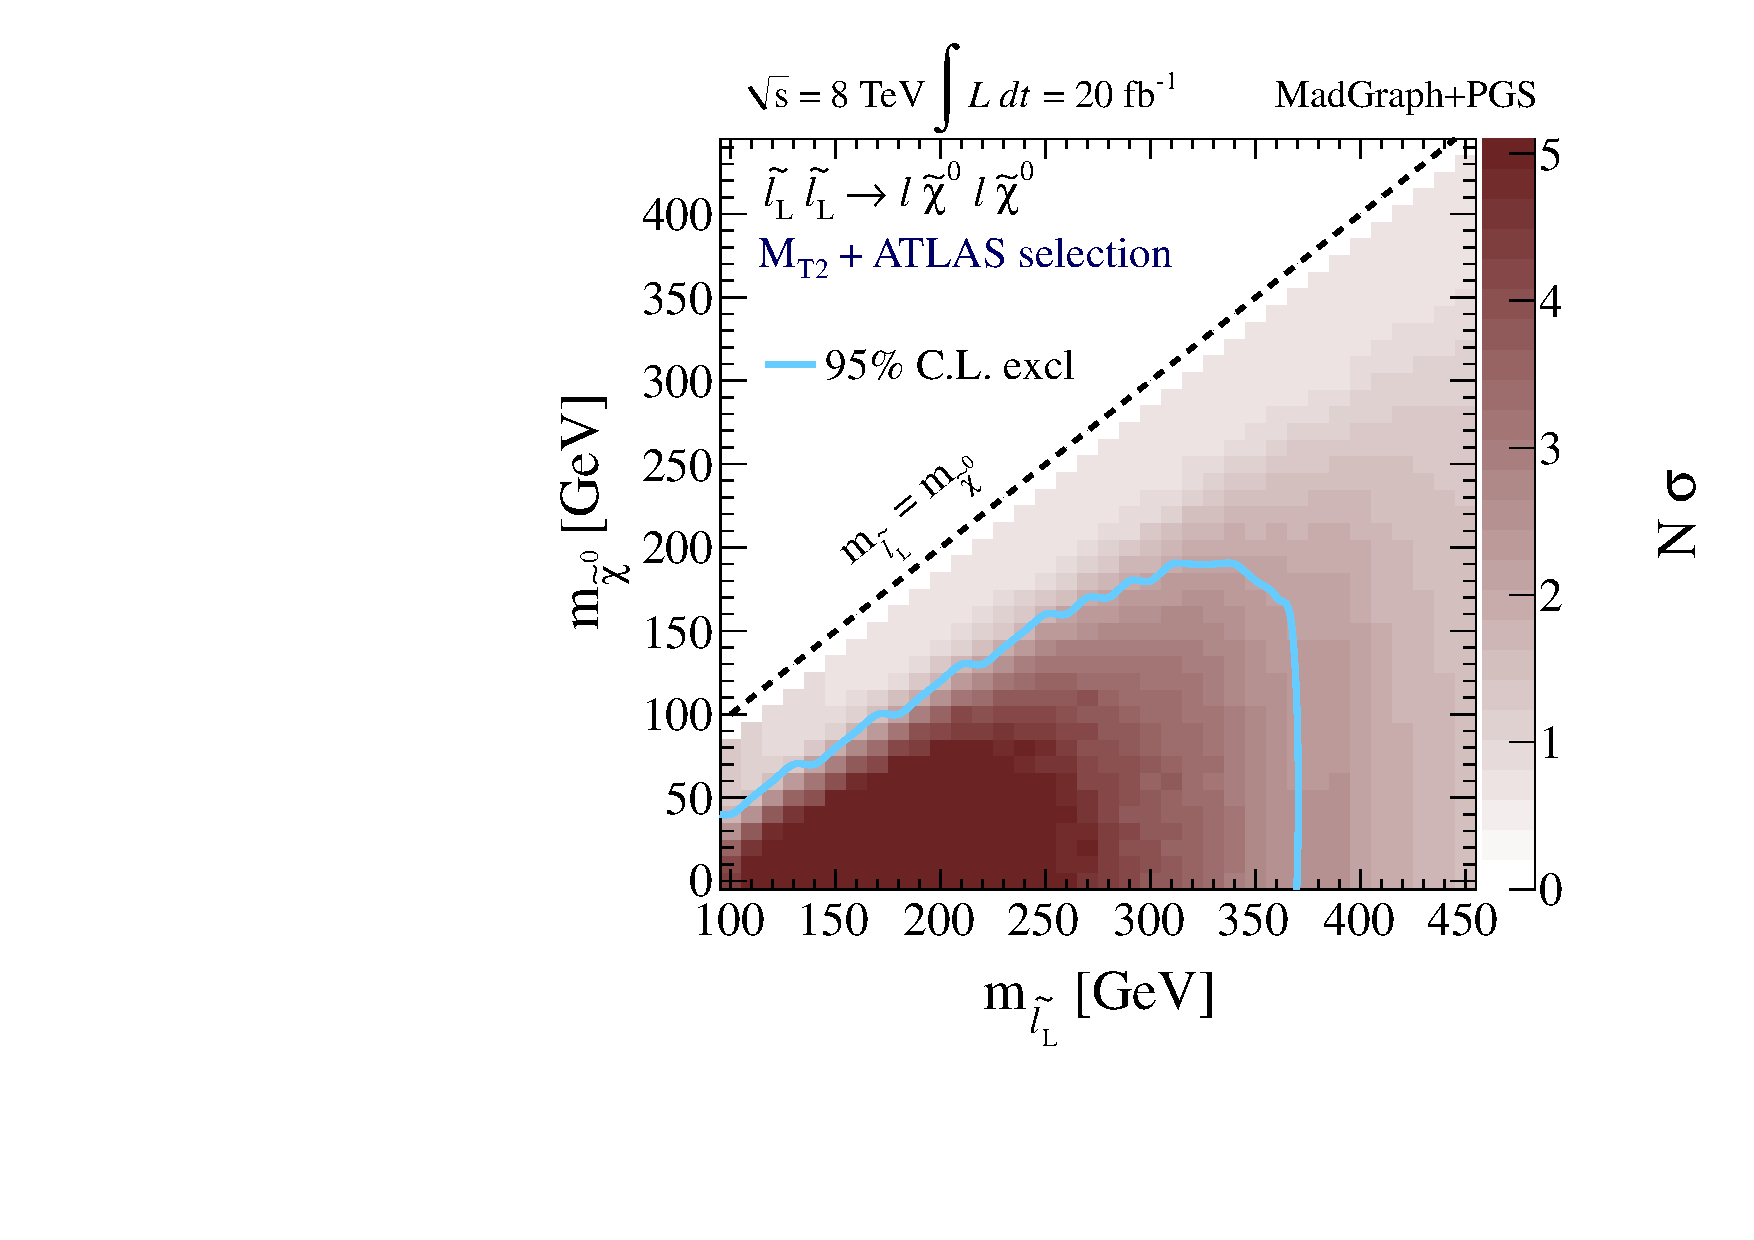
\includegraphics[width=0.35\columnwidth]{fig/sectionIV/LIMIT2D_selectronL_ATLAS_MT2_CLs.pdf}
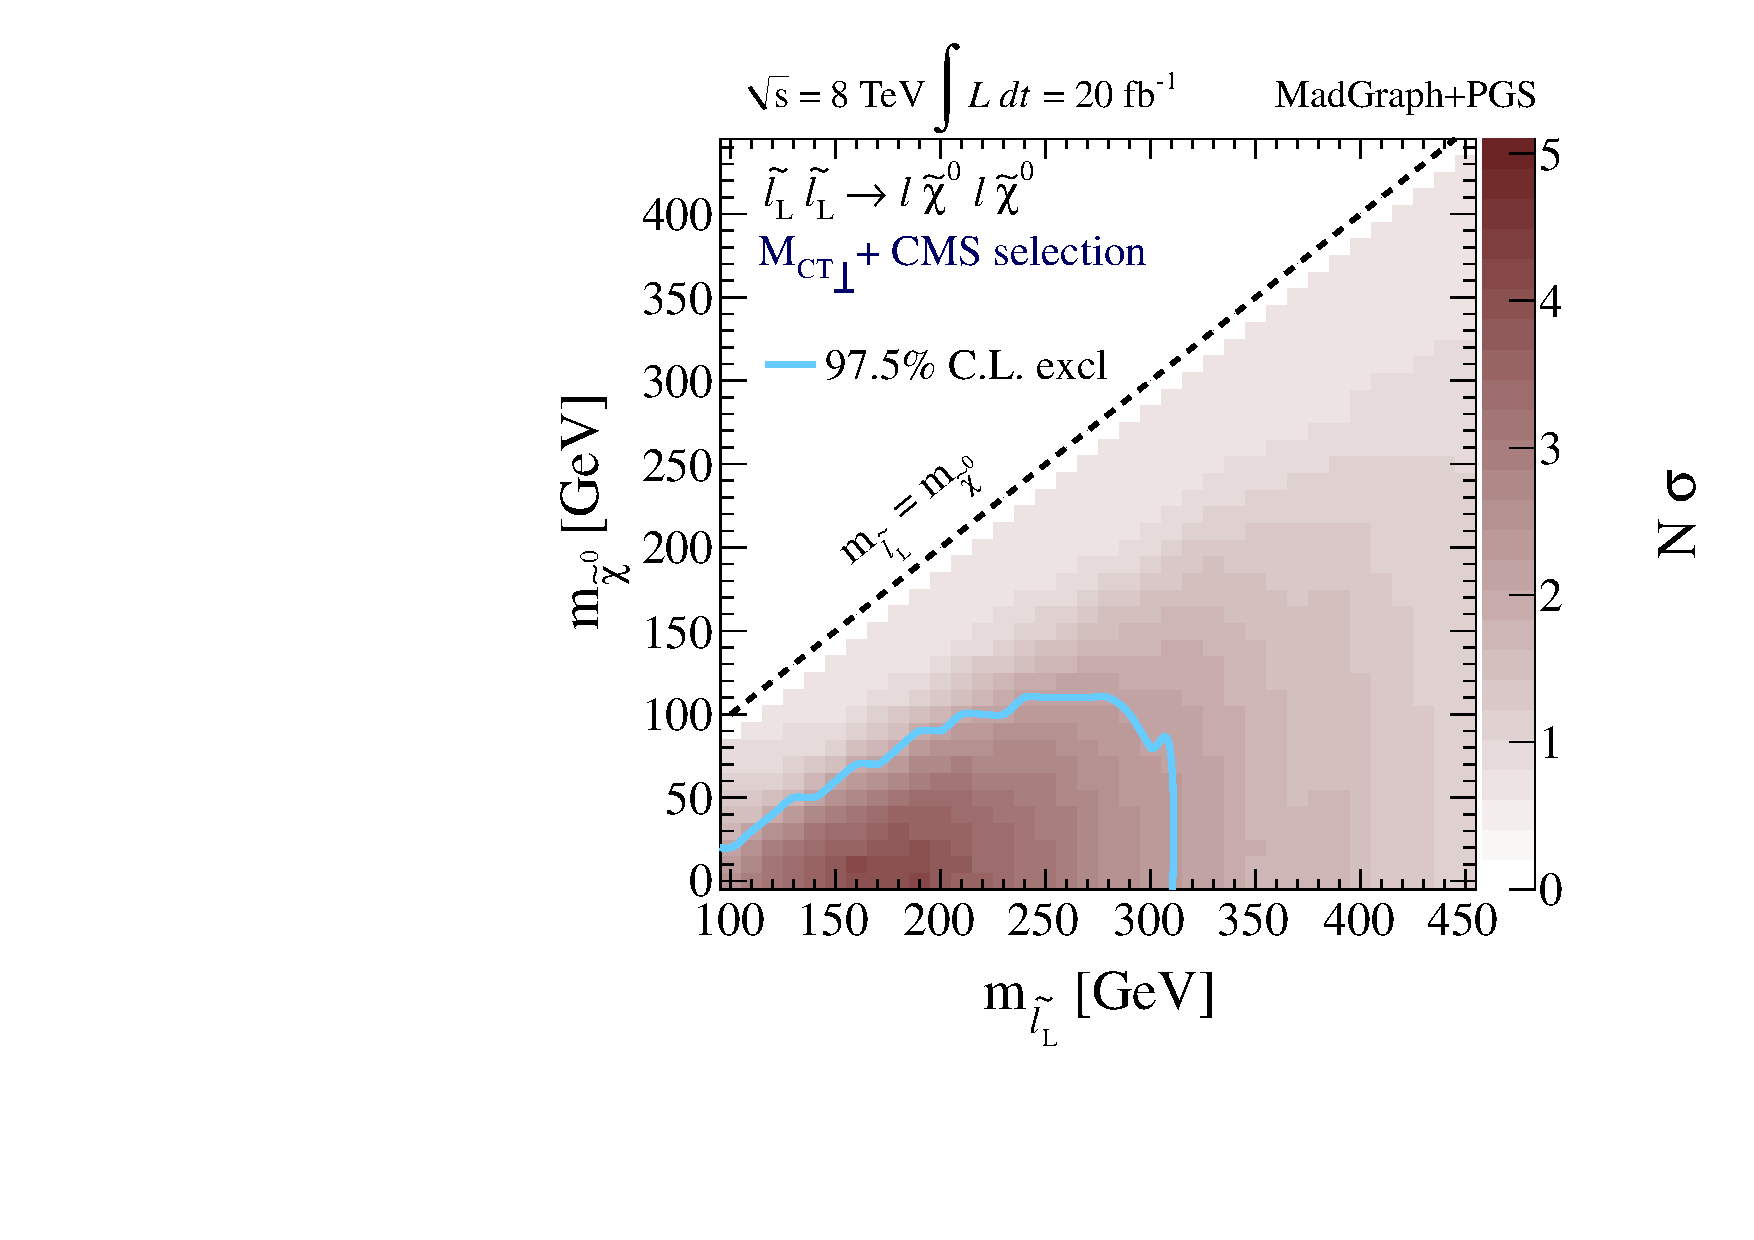
\includegraphics[width=0.35\columnwidth]{fig/sectionIV/LIMIT2D_selectronL_CMS_MCTperp_CLs.pdf}
\caption{ Median expected number of $\sigma$ for excluding the presence of different left-handed di-slepton signals, as a function of slepton and neutralino masses. Left: Expected results using $M_{T2}$ with the ATLAS selection. Right: Expectations when using $M_{CT\perp}$ in conjunction with the CMS selection.\label{fig:CLs} }
\end{figure}

